%%%%%%%%%%%%%%%%%%%%%%%%%%%%%%%%%%%%%%%%%%%%%%%%%%%%%%%%%%%%%%%%%%%%%%%%
\newpage
\section{Sheared and deformed objects}

\subsection{Non-equilibrium static form factor of a reptating chain}
\begin{figure}[htb]
\begin{center}
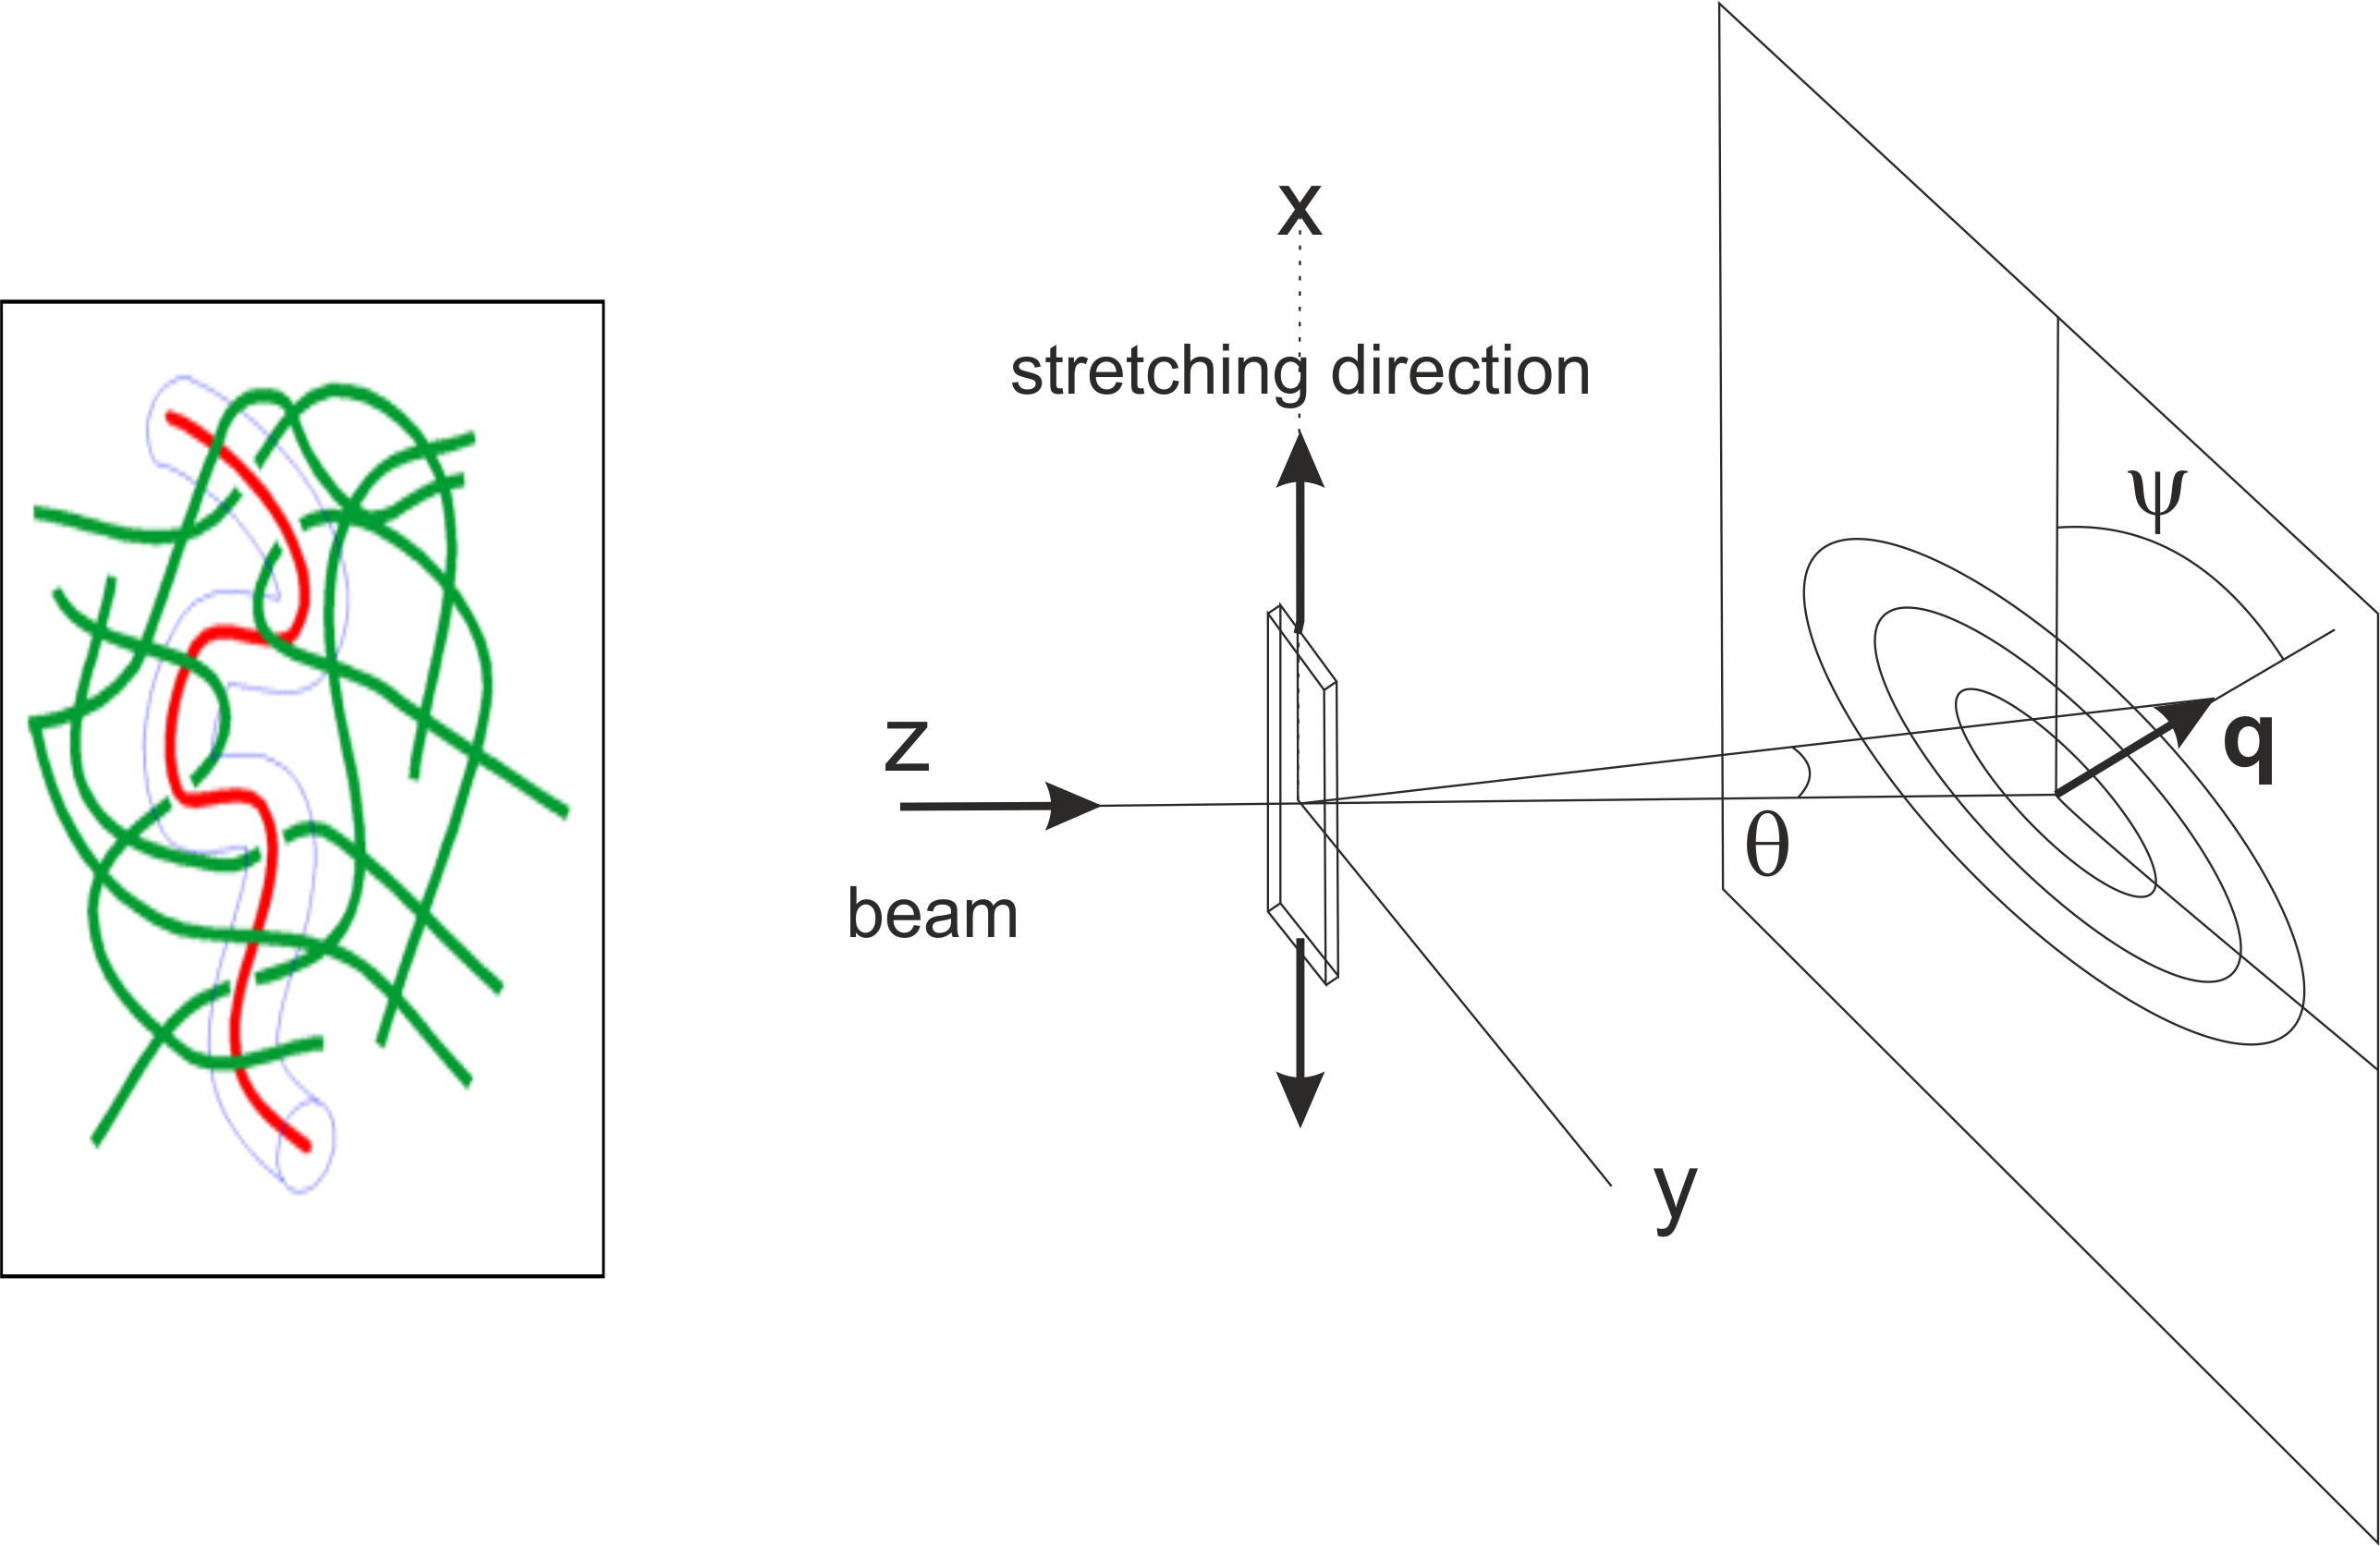
\includegraphics[width=\textwidth]{../images/form_factor/reptating_chain/reptating_chain.png}
\end{center}
\caption{Sketch of experimental setup for stretching a polymer melt.}
\label{fig:stretchpolymermelt}
\end{figure}
This model \cite{Hong1983,Noolandi1984} describes the scattering behaviour of an uniaxial deformed (stretched) Gaussian polymer chain as a function of the deformation ratio and Rouse relaxation time. The model might not include an up-to-date tube model but shows some main features of deformed polymer melts.
\newlength\breites
\settowidth\breites{$\displaystyle {}+{}$}
\begin{align}
\begin{split}
I\left(q,\frac{t}{\tau}\right)/I_0 = & \hspace{\breites}
                                        D(\alpha) + \frac{1}{6}(\alpha-\beta) \left(1+e^{-\alpha}\right) H\left(\alpha,\frac{t}{\tau}\right) \\
                                     & + \frac{1}{6}(\alpha-\beta)^2 e^{-\beta} \int_0^1 \mathrm{d}y \, y^3 e^{\beta y} \left(1+e^{-\alpha y}\right) H\left(\alpha y,\frac{t}{\tau y^2}\right)
\end{split}
\end{align}
with
\begin{align}
H\left(x,\frac{t}{\tau}\right) &= \frac{96}{\pi^2} \sum_{n = \mathrm{odd}} \frac{1}{n^2\left(n^2\pi^2+x^2\right)} e^{-n^2 \frac{t}{\tau}}
\end{align}
$D(x)$ is the Debye function $D(x) = 2\left(x - 1 + e^{-x}\right)/x^2$, $\alpha = q^2 R_g^2$, $R_g$ is the equilibrium radius of gyration
of the chain and $\tau$ is the reptation time or tube disengagement time.
Furthermore $\lambda$ is the uniaxial elongation factor, $q_\parallel$ and $q_\perp$ are respectively the components of the wave vector $q$ in directions parallel and
perpendicular to the direction of elongation which than define the parameter $\beta$ as
\begin{align}
\beta &= \left(q_\parallel^2\lambda^2+q_\perp^2/\lambda\right) R_g^2/E \\
E &= \frac{1}{2} \left\{\lambda +\frac{\mathrm{asinh}\left(\sqrt{\lambda^3-1}\right)}{\sqrt{\lambda\left(\lambda^3-1\right)}} \right\} \\
q_\parallel &= q \cos(\psi-\theta_0) \\
q_\perp &= q \sin(\psi-\theta_0)
\end{align}

\hspace{1pt}\\
\underline{Input Parameters for models \texttt{CylShell1}, \texttt{CylShell2} and \texttt{LongCylShell}:}\\
\begin{description}
\item[\texttt{I0}] forward scattering $I_0$
\item[\texttt{Rg}] radius of gyration of unstretched polymer $R_r$
\item[\texttt{lambda}] stretching factor $\lambda$
\item[\texttt{t/tau}] relaxation time in units of Rouse time $t/\tau$
\item[\texttt{theta\_0}] stretching direction in the detector plane $\theta_0$ in degree
\item[\texttt{psi}] $\mathbf{q}$-direction $\psi$ in the detector plane in degree
\end{description}

\underline{Note:}
\begin{itemize}
\item The model only converges for $\lambda >1$.
\end{itemize}

\begin{figure}[htb]
\begin{center}
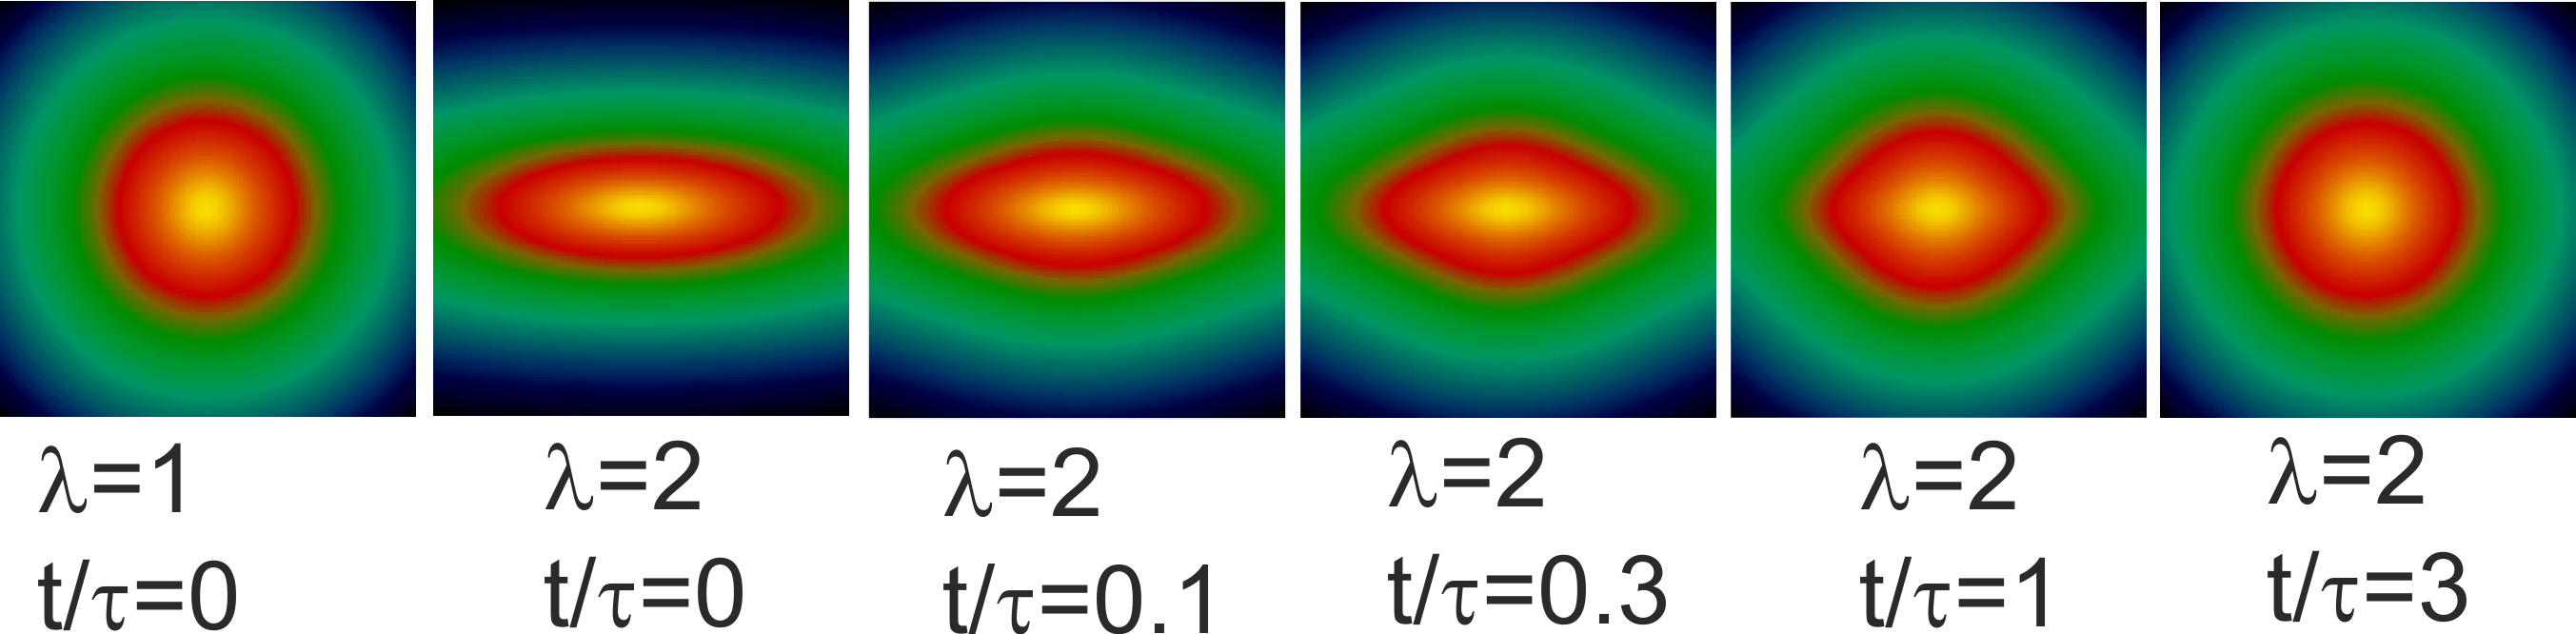
\includegraphics[width=\textwidth]{../images/form_factor/reptating_chain/lambda_2_reptating_chains.png}
\end{center}
\caption{2D scattering patterns for different relaxation times $t/\tau$ after a deformation step of $\lambda=2$}
\label{fig:IQ2Dstretchedpolymermelt}
\end{figure}

%%%%%%%%%%%%%%%%%%%%%%%%%%%%%%%%%%%%%%%%%%%%%%%%%%%%%%%%%%%%%%%%%%%%%%%%%
\newpage
\subsection{ShearedCylinderHayterPenfold}
\label{sect:ShearedCylinderHayterPenfold}
\hspace{1pt}\\
The orientation distribution of long cylinders in a shear cell has been studied by \cite{Scheraga1951,Jerrard1959,Hayter1984}. In contrast to the orientation distributions described in the next section this distribution also describes the tilting of the most probable orientation against the flow direction.
\begin{figure}[htb]
\begin{center}
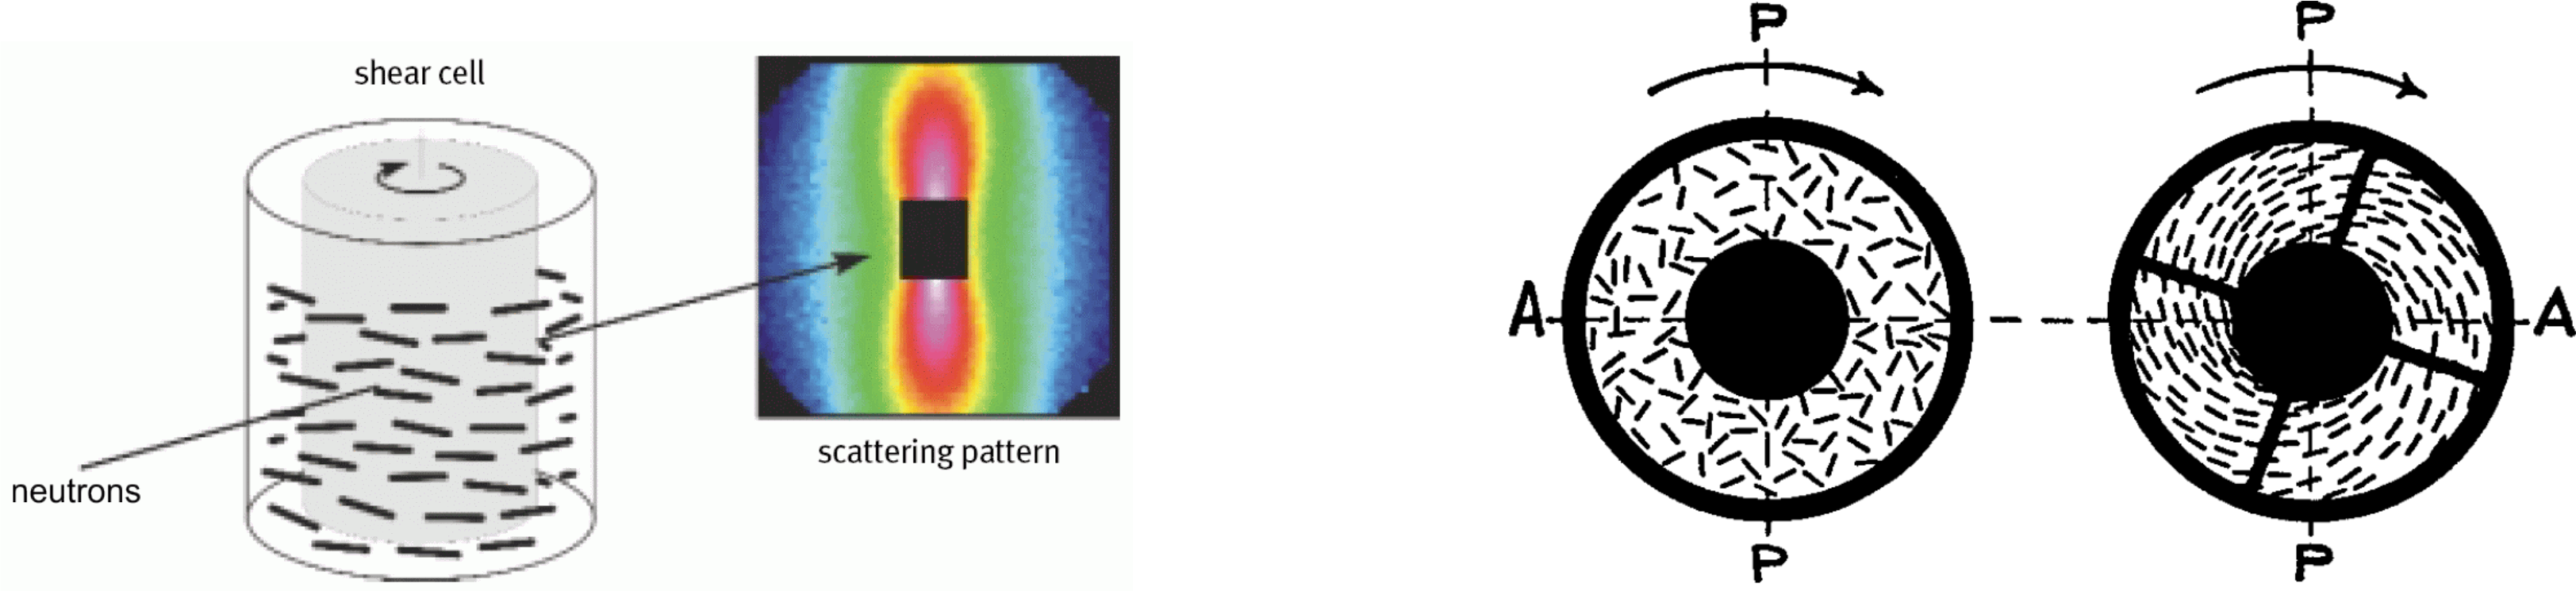
\includegraphics[width=\textwidth]{sheared_cylinders_n_phi0.png}
\end{center}
\caption{Shear orientation of micelles in a shear cell with the
corresponding SANS-pattern. The orientation of rods at rest and under shear according to \cite{Scheraga1951} are shown on th e right as a top view on the cuette cell.} \label{sheared_cylinders1}
\end{figure}

\begin{figure}[htb]
\begin{center}
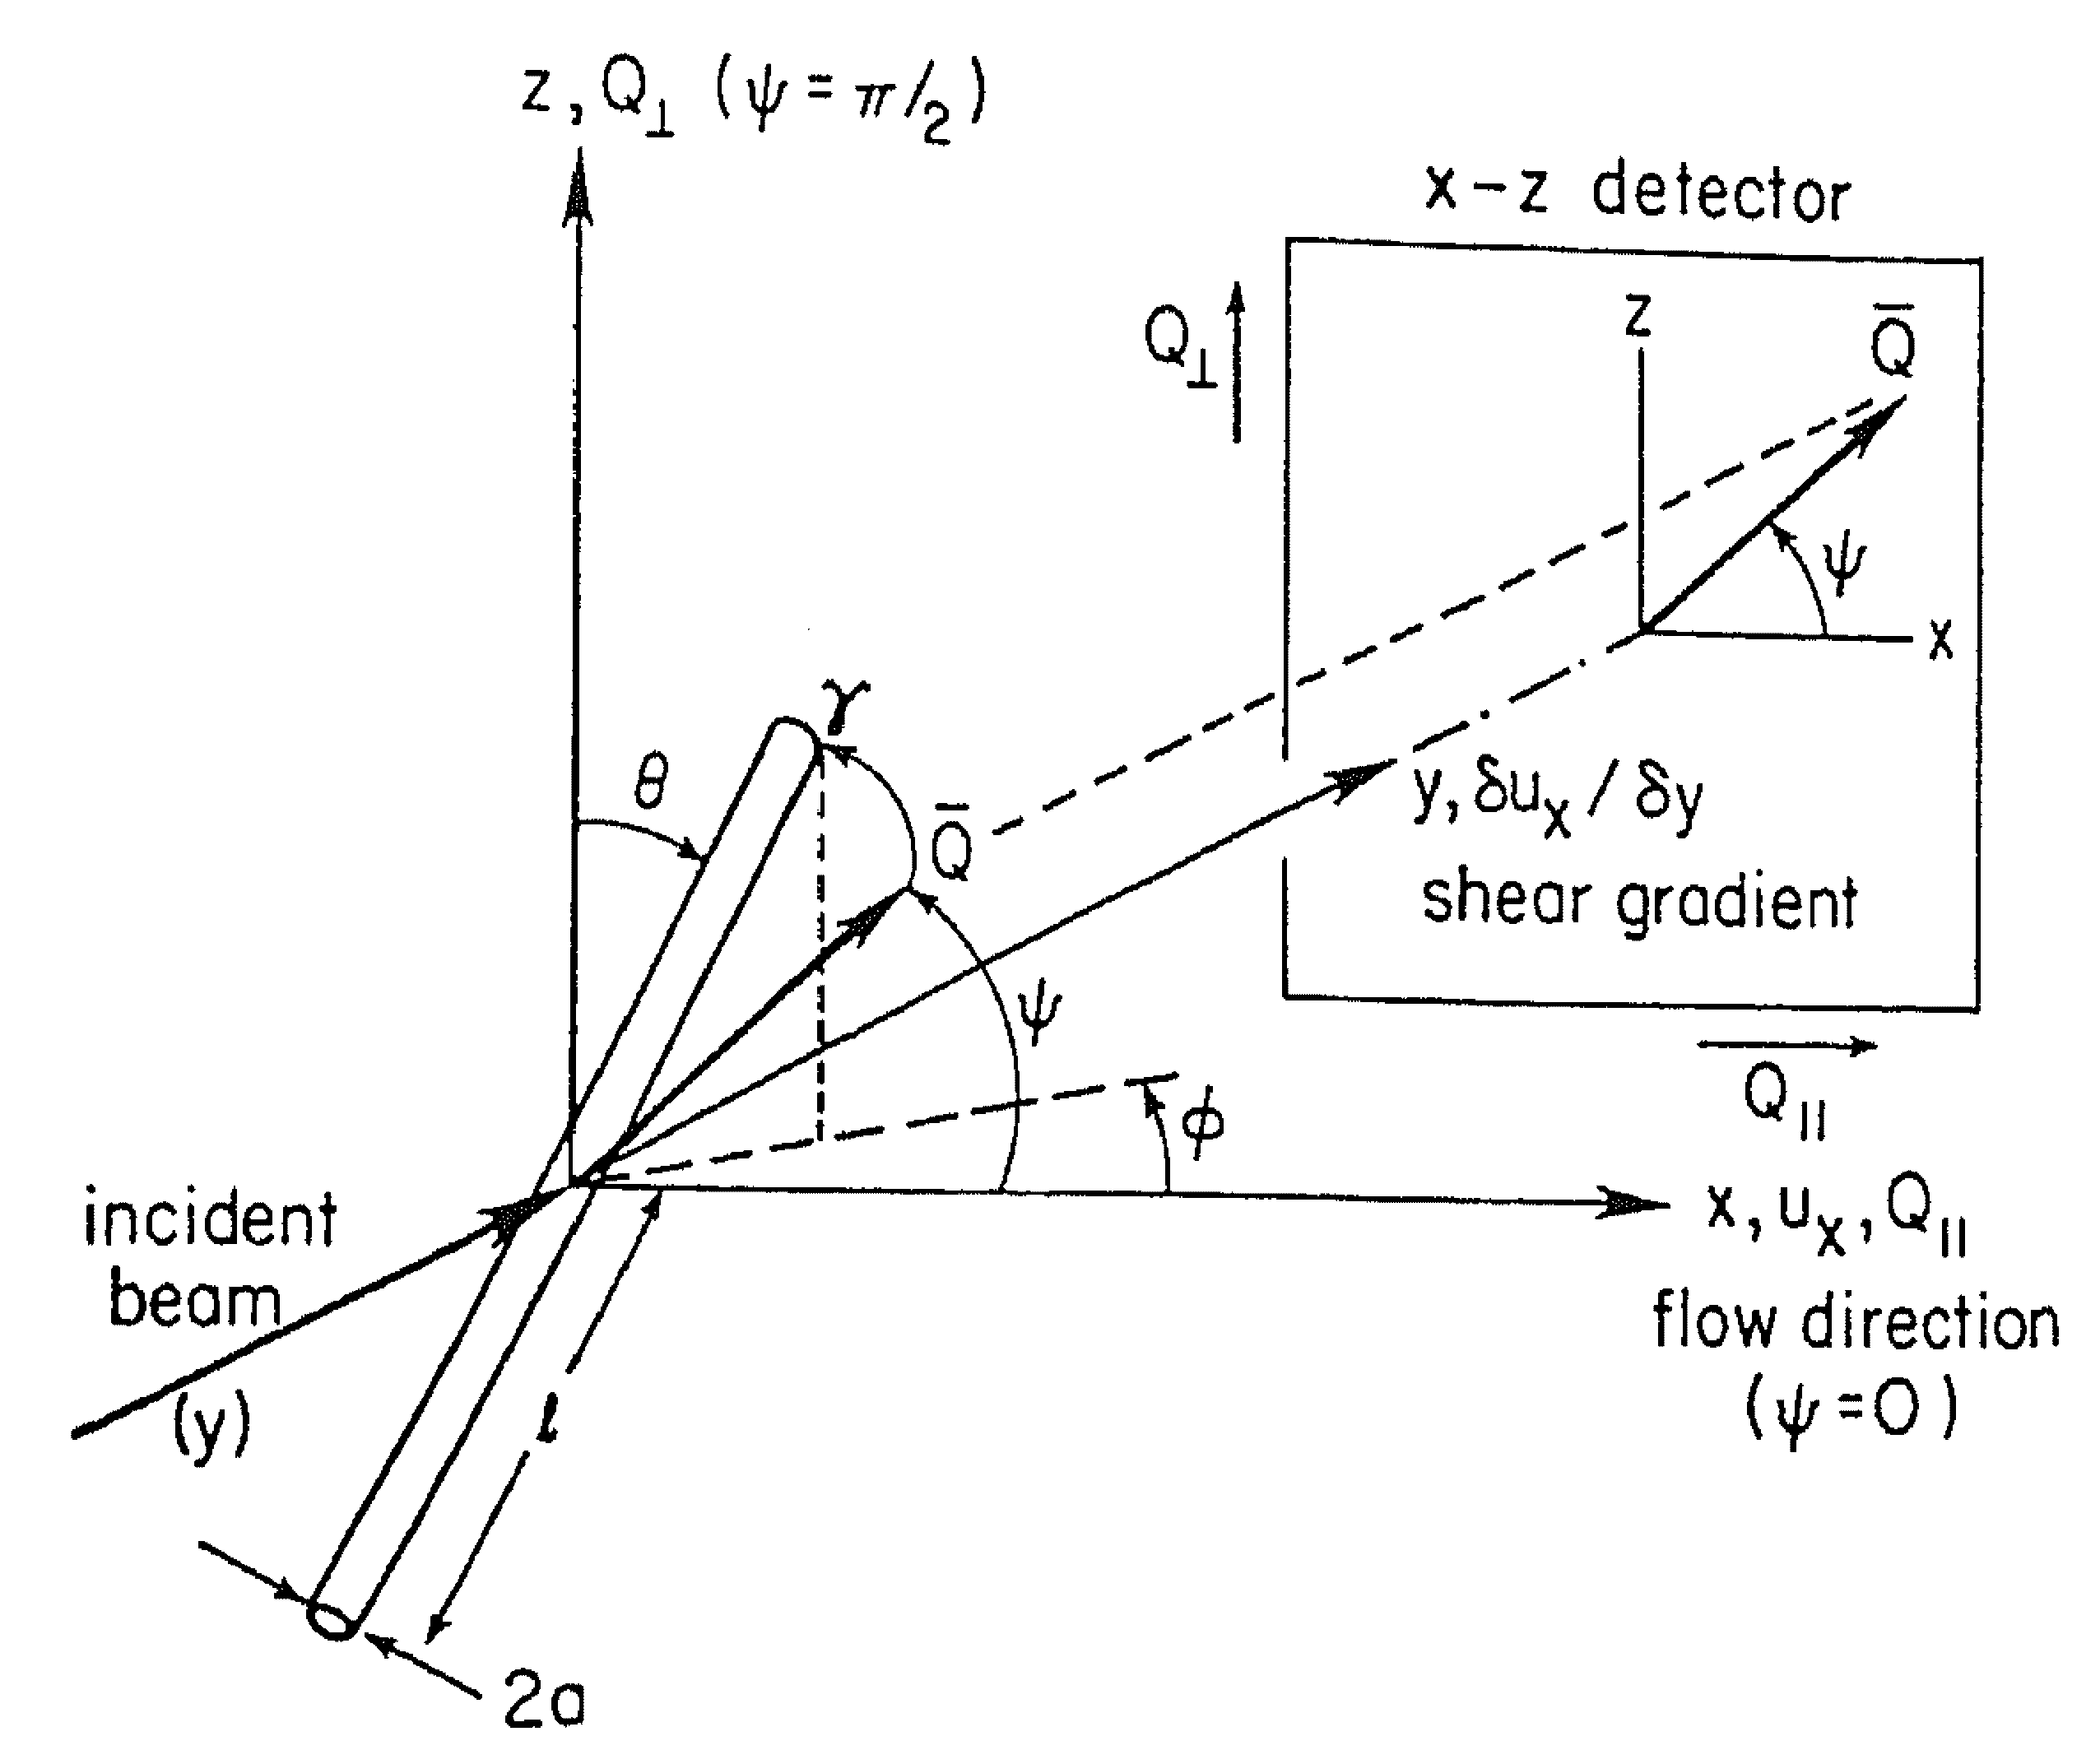
\includegraphics[width=0.7\textwidth]{shear_cuette_SANS_geometry.png}
\end{center}
\caption{Cartesian and angular coordinates referred to the center
of a cylindrical micelle at origin \cite{Hayter1984}. The relationship to the
spectrometer geometry is shown schematically. The momentum
transfer, $Q$, lies in the $z-x$ plane.}
\label{shear_cuette_SANS_geometry}
\end{figure}

The scattering from monodisperse dilute (non-interacting)
isotropic solution of anisotropic micelles is given by \cite{Hayter1984}
\BE
I(Q) =
\left< \vert F(Q)\vert^2 \right>_Q \label{IQ_av}
\EE
where $F(Q)$
is the form factor for a micelle at a given orientation relative
to the momentum transfer $Q$ and $\left<\right>_Q$ denotes an
average over all such orientations.

For a uniform cylinder of length $L$ and diameter $2R$ the form
factor is given by:
\BE F(Q) = F(Q,\gamma) = 2\Delta\eta V
\frac{\sin\left(QL/2\cos\gamma\right)}{QL/2\cos\gamma}
\frac{J_1(QR\sin\gamma)}{QR\sin\gamma}
\EE
where $\gamma$ is the
angle between $Q$ and the cylinder axis, $V$ is the volume,
$\Delta\eta$ the scattering length density contrast relative to
the solvent, $J_1(x)$ is the first order Bessel function of the
first kind.

The scattering geometry for shear alignment is shown in Fig.
\ref{shear_cuette_SANS_geometry}. In general perfect alignment
will not be achieved, and an orientation distribution must be
employed such that the resultant scattering will be given by
\begin{align}
I(Q,\psi) &= \int_0^{2\pi} \int_0^\pi
p_\mathrm{HP}(\theta,\phi;\kappa)\, \left(F^2(Q,\gamma^+)+F^2(Q,\gamma^-)
\right) \sin\theta \mathrm{d}\theta \mathrm{d}\phi
\label{eq:IQShear_pHP}
\end{align}
with
\begin{align}
p_\mathrm{HP}(\theta,\phi;\kappa) & = \frac{(1-\cos
2\varPhi_0)(1+\sin^2\theta\cos 2\varPhi_0)^{3/2}}{4\pi\left[
1-\sin^2\theta\cos 2\varPhi_0\cos 2(\phi-\varPhi_0)\right]^2}
\end{align}
and
\BE
2\varPhi_0 = \arctan(8/\kappa)
\EE
$(\cos \varPhi_0,\sin \varPhi_0,0)^T$
is the direction of the most probable orientation $(\theta=\frac{\pi}{2};\phi=\varPhi_0)$. $\varPhi_0$ varies between $\varPhi_0=\frac{\pi}{4}$ for the isotropic case ($\kappa=0$)  to $\varPhi_0=0$ for perfect alignment ($\kappa\rightarrow \infty$).
\begin{figure}[htb]
\begin{center}
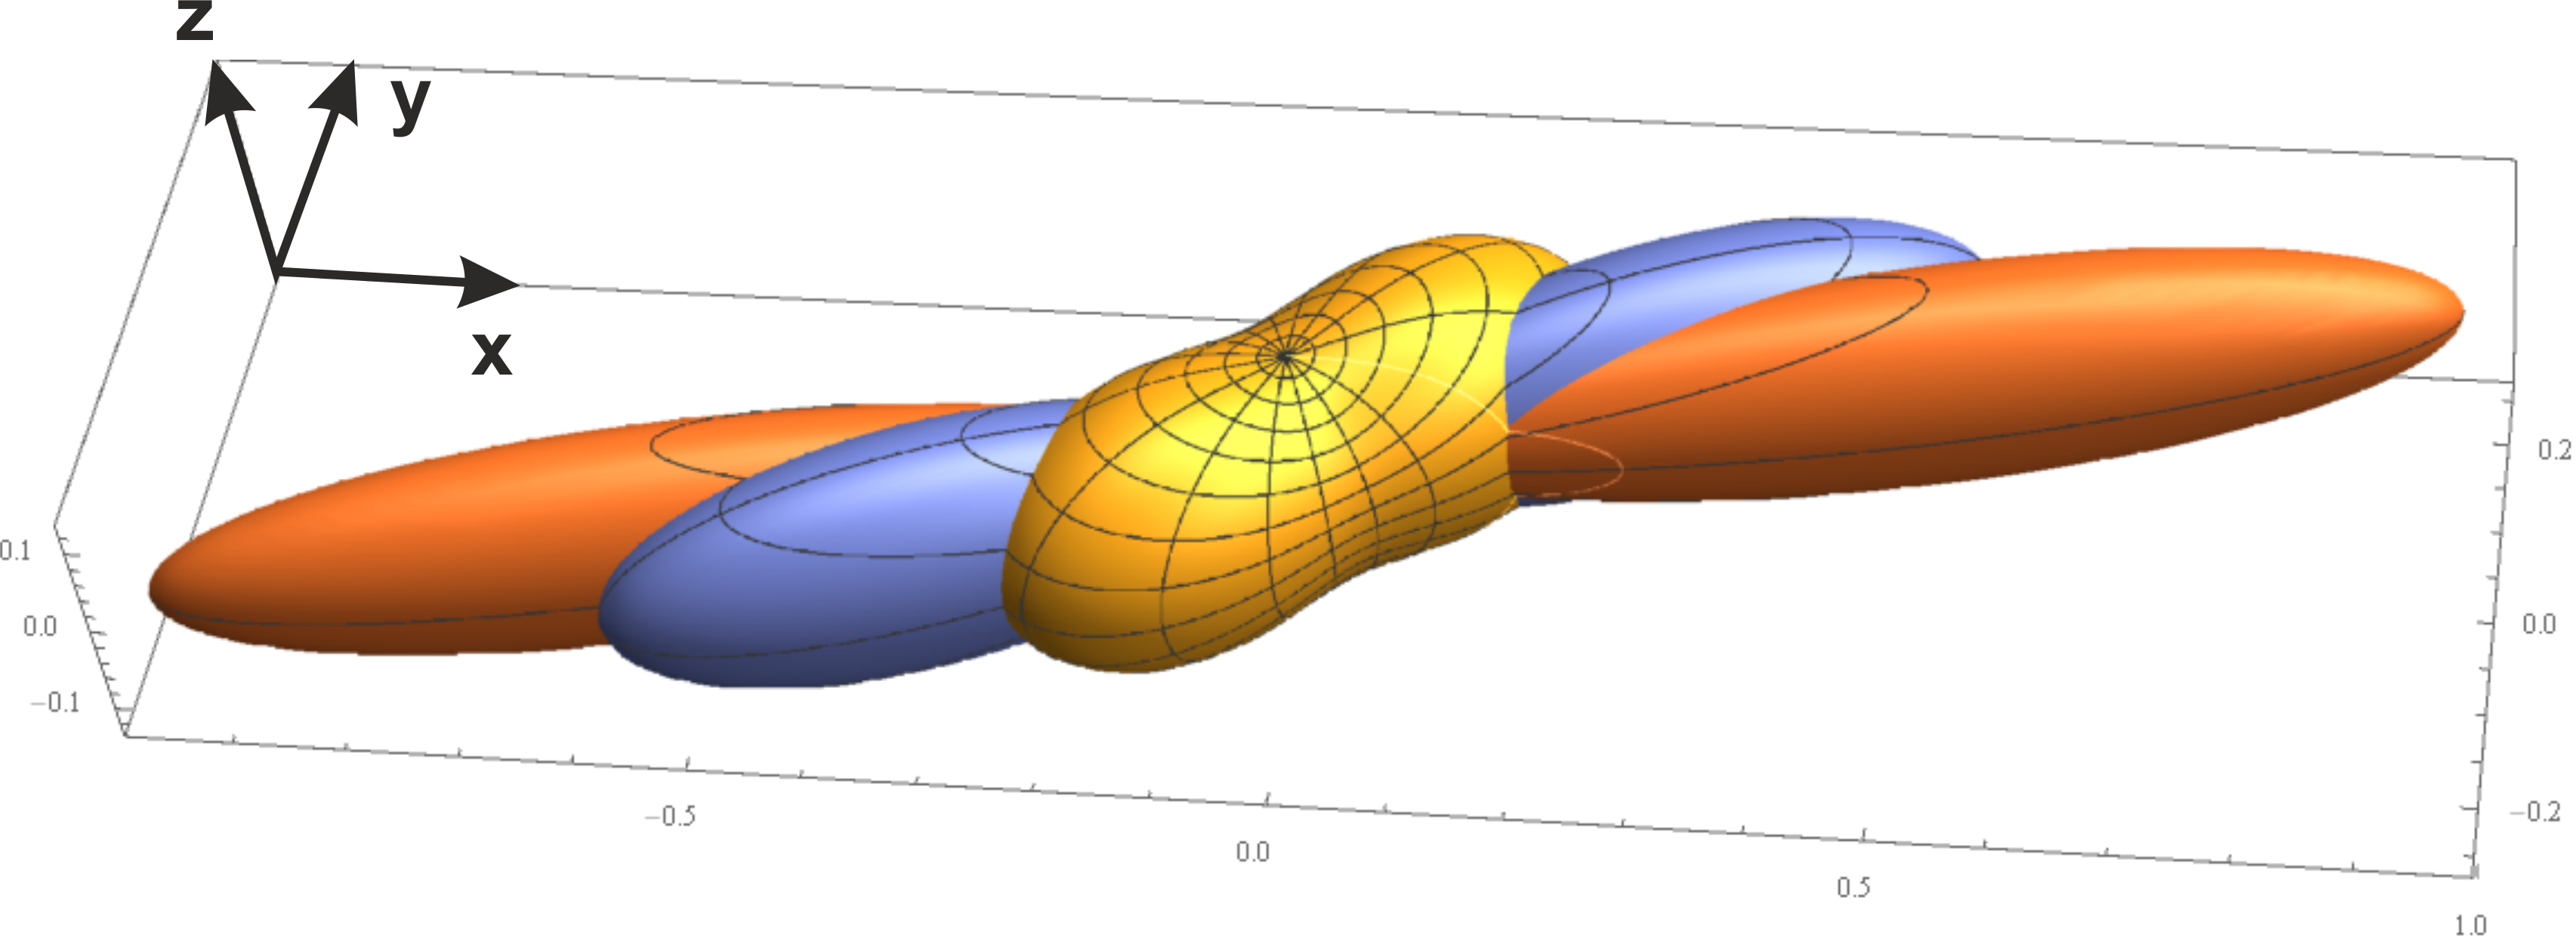
\includegraphics[width=\textwidth]{../images/form_factor/cylindrical_obj/pHP3D.png}
\end{center}
\caption{3D plot of the orientation distributions $2 p_\mathrm{HP}(\theta,\phi;\kappa={2})$ ({\bf \color[rgb]{1.0, 0.85, 0.0}yel-}{\bf \color[rgb]{1.0, 0.85, 0.0}low}), $p_\mathrm{HP}(\theta,\phi;\kappa{=}8)$ ({\bf\color[rgb]{0.36, 0.57, 0.9} blue}), $\frac12 p_\mathrm{HP}(\theta,\phi;\kappa{=}16)$ ({\bf\color[rgb]{1.0, 0.5, 0.0} orange}).} \label{fig:pHP3D}
\end{figure}
As the most probable direction is not the same as the flow direction, which is assumed to be the $x$-direction, and secondly that the beam is passing twice the cuette cell with flow direction $\mathbf{x}$ and $-\mathbf{x}$ we have to take the sum over two values for $\gamma^\pm$ in eq.\ \ref{eq:IQShear_pHP}. The angle $\gamma^\pm = \angle(\mathbf{Q,n}^\pm)$ between the scattering vector $\mathbf{Q}$ and the director of the cylinder axis $\mathbf{n}^\pm$ is
\begin{align}
\frac{\mathbf{Q}}{\abs{\mathbf{Q}}} &=
\begin{pmatrix}
\cos \psi \\
0  \\
\sin \psi
\end{pmatrix} \qquad
\frac{\mathbf{n}^\pm}{\abs{\mathbf{n}^\pm}} =
\begin{pmatrix}
\pm \sin \theta \cos \phi \\
\pm \sin \theta \sin \phi  \\
\cos \theta
\end{pmatrix} \\
\cos \angle(\mathbf{Q,n}^\pm) &= \cos \gamma^\pm = \frac{\mathbf{Q\cdot n}^\pm}{\abs{\mathbf{Q}}\abs{\mathbf{n}^\pm}} =  \pm \cos\psi \sin\theta \cos\phi + \sin\psi \cos\theta
\end{align}
For the reversed direction of the flow the $x$-component of the vector $\mathbf{n}^-$ changes its sign. In the original paper \cite{Hayter1984} one finds $\cos \gamma^-_\mathrm{HP} = \cos\psi \sin\theta \cos\phi - \sin\psi \cos\theta$, which, however, results to the same scattering intensity as the scattering intensity of a cylinder is invariant by a rotation of $\pi$, i.e. as $\cos(\pi+\gamma^-) =-\cos\gamma^- = \cos\gamma^-_\mathrm{HP}$ the resulting scattering patterns are the same for both value $\gamma^-$ and $\gamma^-_\mathrm{HP}$.

%%%%%%%%%%%%%%%%%%%%%%%%%%%%%%%%%%%%%%%%%%%%%%%%%%%%%%%%%%%%%%%%%%%%%%%%%%%%%%%%%%
\newpage
\subsection{partly aligned cylindrical shell}
\label{sect:partlyalignedCylShell}
~\\

In contrast to the model of Hayter and Penfold \cite{Hayter1984} in section \ref{sect:ShearedCylinderHayterPenfold} here we use an orientation distribution with the most probably orientation along the $\mathrm{x}$-axis and independent on the polar angle $\phi$.
Therefore the coordination system is slightly differently defined in the Hayter-Penfold model of sheared cylinders.
\begin{figure}[htb]
\begin{center}
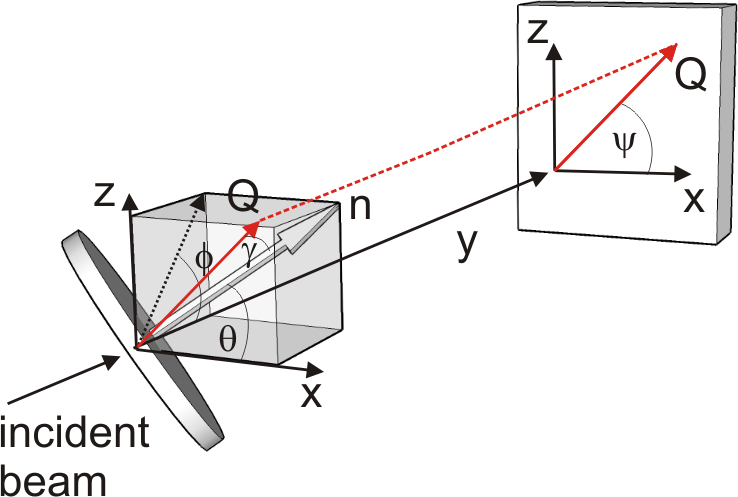
\includegraphics[width=0.7\textwidth]{../images/form_factor/cylindrical_obj/partly_aligned_discs.png}
\end{center}
\caption{Sketch of relative orientation $\mathbf{n}$ of partly
aligned cylinders or discs to the scattering vector $\mathbf{Q}$.}
\label{fig:partly_aligned_discs}
\end{figure}

\noindent The scattering amplitude of a cylindrical shell is given by
\begin{align}
K_\text{CylShell}\left(Q,\dots,\gamma\right)  = &K_\text{Cyl}\left(Q,\eta_\text{core}-\eta_\text{shell},R,L,\gamma\right) \\
& +  K_\text{Cyl}\left(Q,\eta_\text{shell}-\eta_\text{solv},R+\Delta
R,L,\gamma\right)
\end{align}
with
\begin{align}
K_\text{Cyl}(Q,\Delta\eta,R,L,\gamma) & = 2 \pi R^2 L \Delta \eta
    \frac{J_1\left(Q R \sin\gamma\right)}{Q R \sin\gamma} \,
    \frac{\sin\left(\frac{QL}{2} \cos\gamma\right)}{\frac{QL}{2} \cos\gamma}
\end{align}
where $\gamma$ is the angle between $\mathbf{Q}$ and the cylinder
axis $\mathbf{n}$. $L$ is the length of the cylinder, $R$ its
radius, $\Delta\eta$ the scattering length density contrast relative
to the solvent and $J_1(x)$ is the first order Bessel function of
the first kind. $\gamma$ can be calculated from the orientation
($\theta$, $\phi$) of the cylinder and the direction of the
scattering vector $\psi$ in the plane of the detector by
\begin{align}
\frac{\mathbf{Q}}{\abs{\mathbf{Q}}} &=
\begin{pmatrix}
\cos \psi \\
0  \\
\sin \psi
\end{pmatrix} \qquad
\frac{\mathbf{n}}{\abs{\mathbf{n}}} =
\begin{pmatrix}
\cos \theta \\
\sin \theta \cos \phi  \\
\sin \theta \sin \phi
\end{pmatrix} \\
\cos \measuredangle(\mathbf{Q,n}) &= \cos \gamma = \frac{\mathbf{Q\cdot
n}}{\abs{\mathbf{Q}}\abs{\mathbf{n}}} = \cos\psi \cos\theta +
\sin\psi \sin\theta \sin\phi
\end{align}
If the orientation distribution of the orientation vector $\mathbf{n}$ is described by $p(\theta,\phi)$
so that the scattering intensity is given by
\begin{align}
I_\mathrm{p.a.CylShell}(Q) & =
            \int_0^\pi d\theta \int_0^{2\pi} d\phi \, \,
                K_\text{CylShell}\left(Q,\dots,\gamma\right)\,p(\theta,\phi;\kappa)\,\sin(\theta)
\end{align}
For this form factor it is assumed that the orientation distribution is independent of $\phi$,
i.e. $p(\theta,\phi;\kappa)=p(\theta;\kappa)$ and that $p(\theta;\kappa)=p(\pi-\theta;\kappa)$, which means that turning the cylinder by 180$^\circ$ results in the same scattering intensity.
Several orientation distributions have been implemented in a way that their resulting order parameter $S_2$ can have values between -0.5 and 1, which correspond to perfect alignment perpendicular to the $\mathrm{x}$ axis and perfect alignment parallel to it. all probability distributions have been normalized so that
\begin{align}
\int_0^\pi \int_0^{2\pi} p(\theta,\phi;\kappa) \sin \theta \, d\theta \, d\phi&=1
\end{align}
\begin{figure}[htb]
\begin{center}
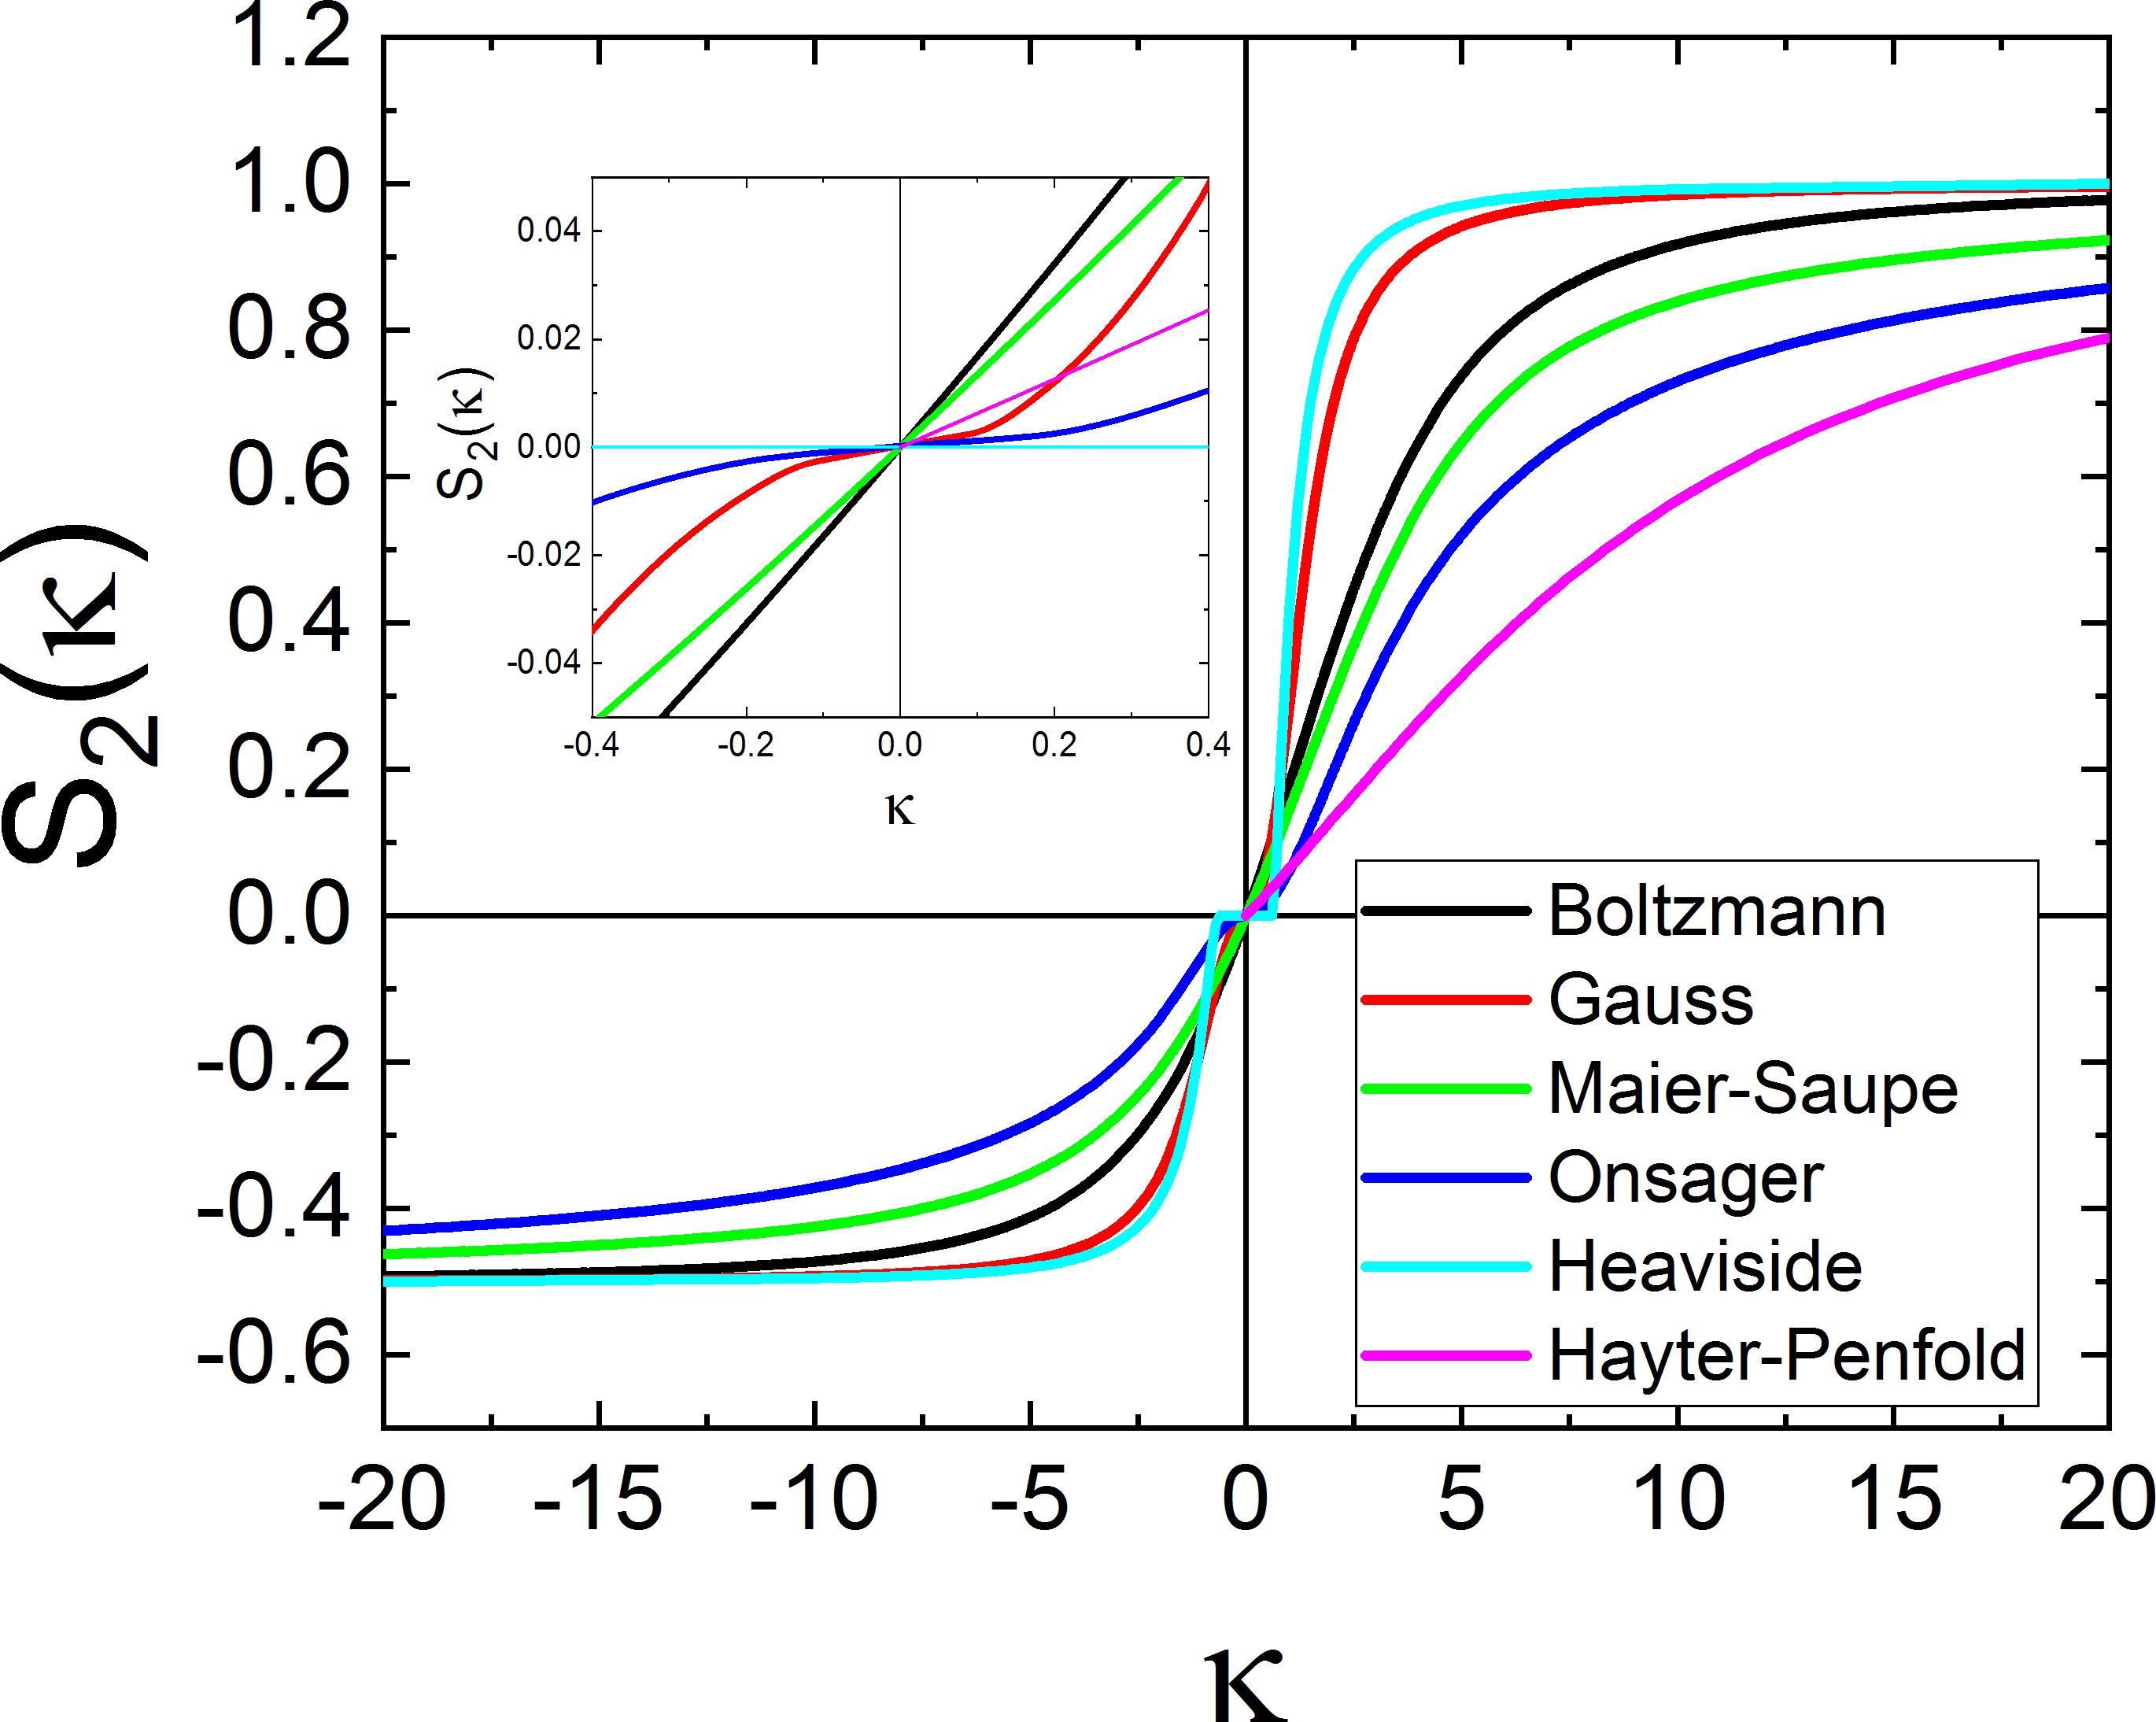
\includegraphics[width=0.75\textwidth]{../images/form_factor/cylindrical_obj/S2(kappa).png}
\end{center}
\caption{Order parameter $S_2(\kappa)$ for the orientation distributions described in the next subsections.}
\label{fig:S2_kappa}
\end{figure}

The order parameters $S_2$ can be calculated by
\begin{align}
S_2(\kappa) &=
\int_0^\pi \int_0^{2\pi}
                p(\theta,\phi;\kappa) \frac12 \left(3\cos^2\theta - 1\right) \sin \theta \, \mathrm{d}\theta\, \mathrm{d}\phi \nonumber \\
&= \int_0^\pi 2\pi
                p(\theta;\kappa) \frac12 \left(3\cos^2\theta - 1\right) \sin \theta \, \mathrm{d}\theta
\end{align}
\begin{figure}[htb]
\subfigure[Onsager orientation distribution for $\kappa=3$. ]{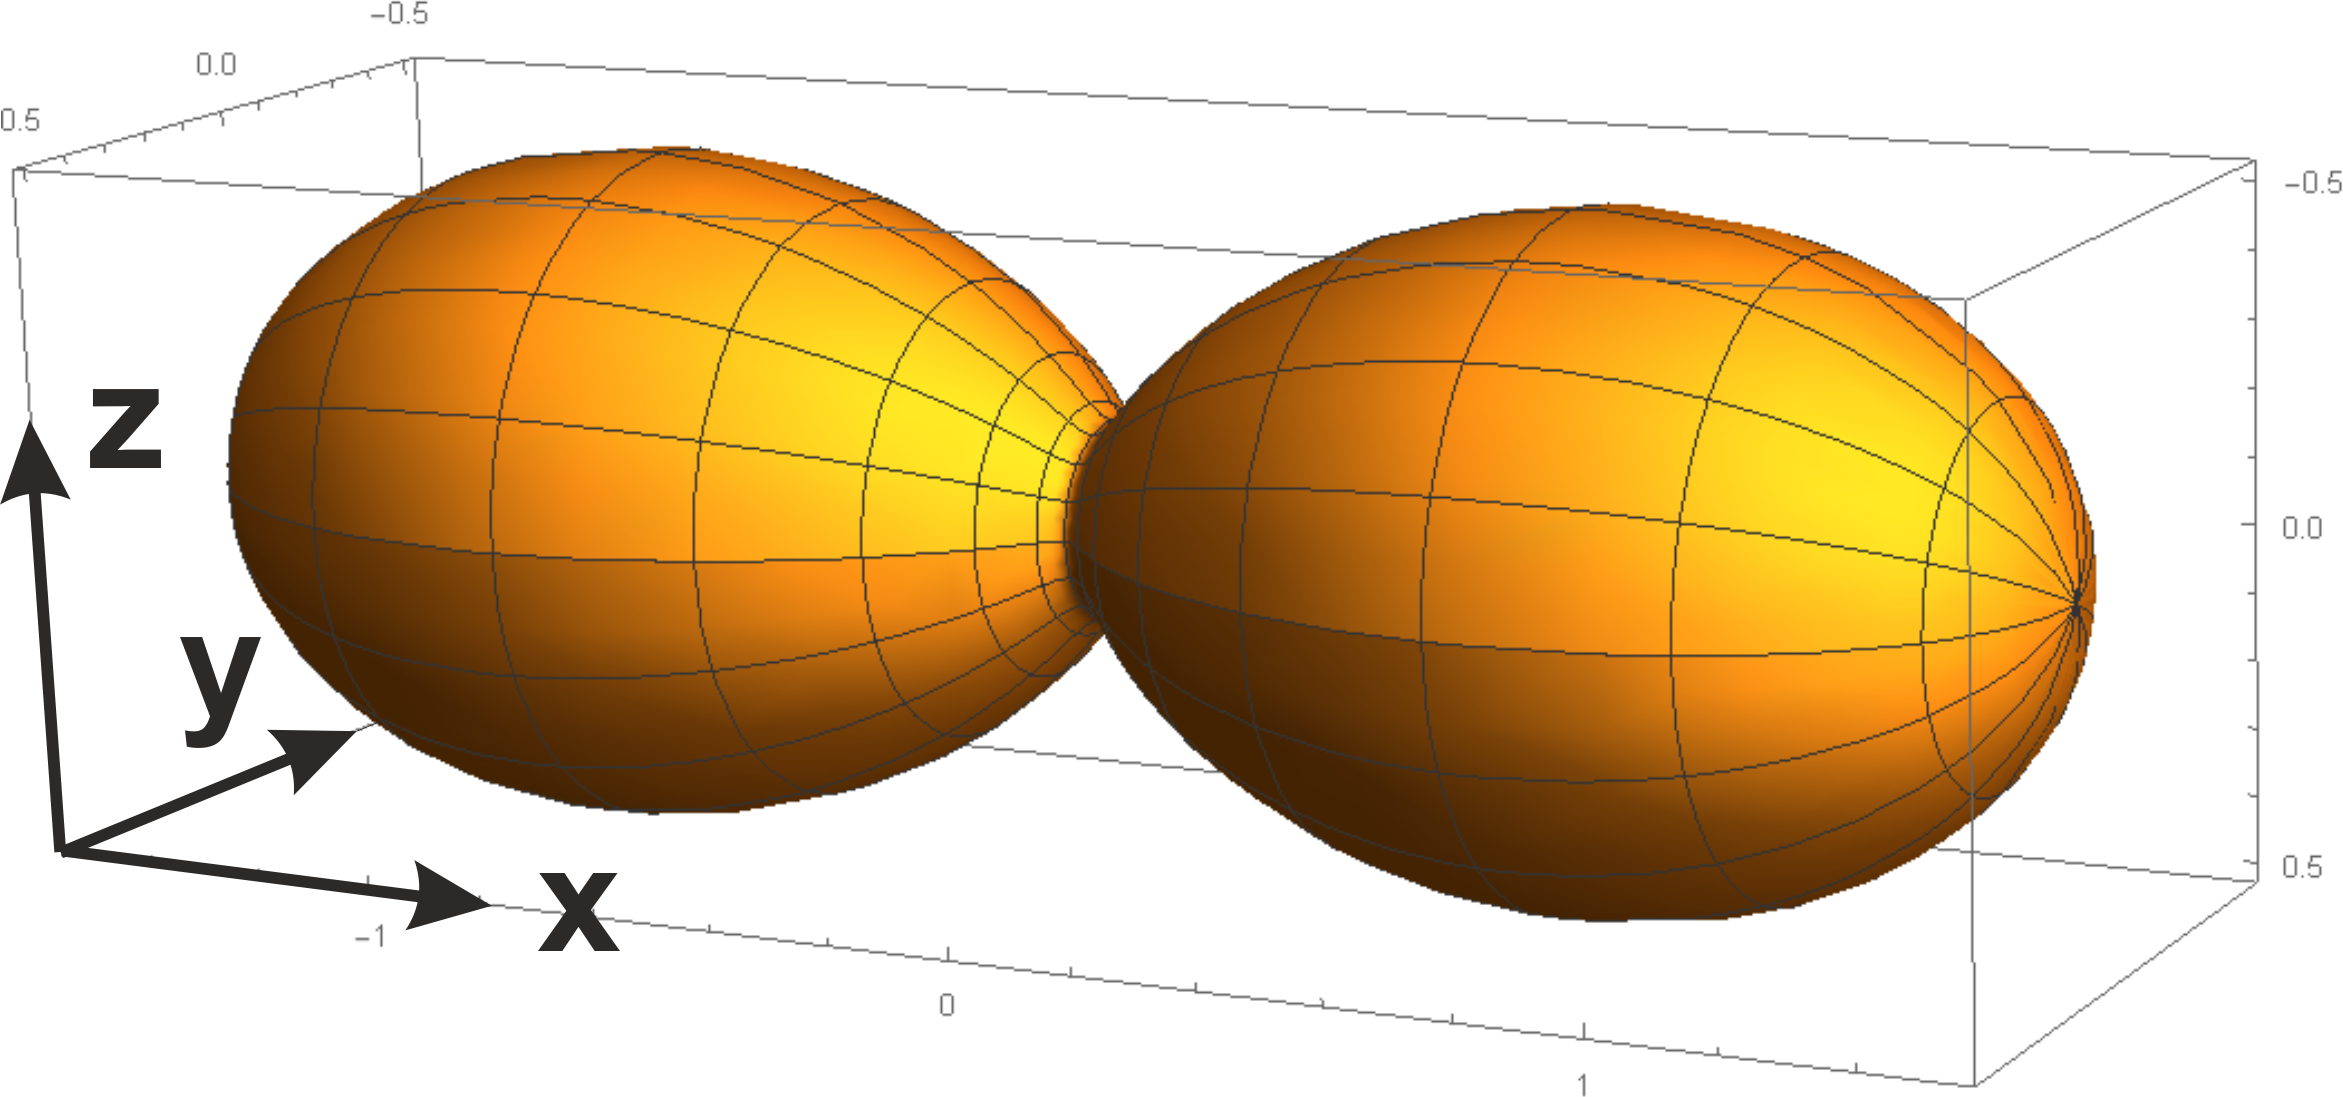
\includegraphics[width=0.55\textwidth]{../images/form_factor/cylindrical_obj/pOnsager(3).png}}
\hfill
\subfigure[Onsager orientation distribution for $\kappa=-3$. ]{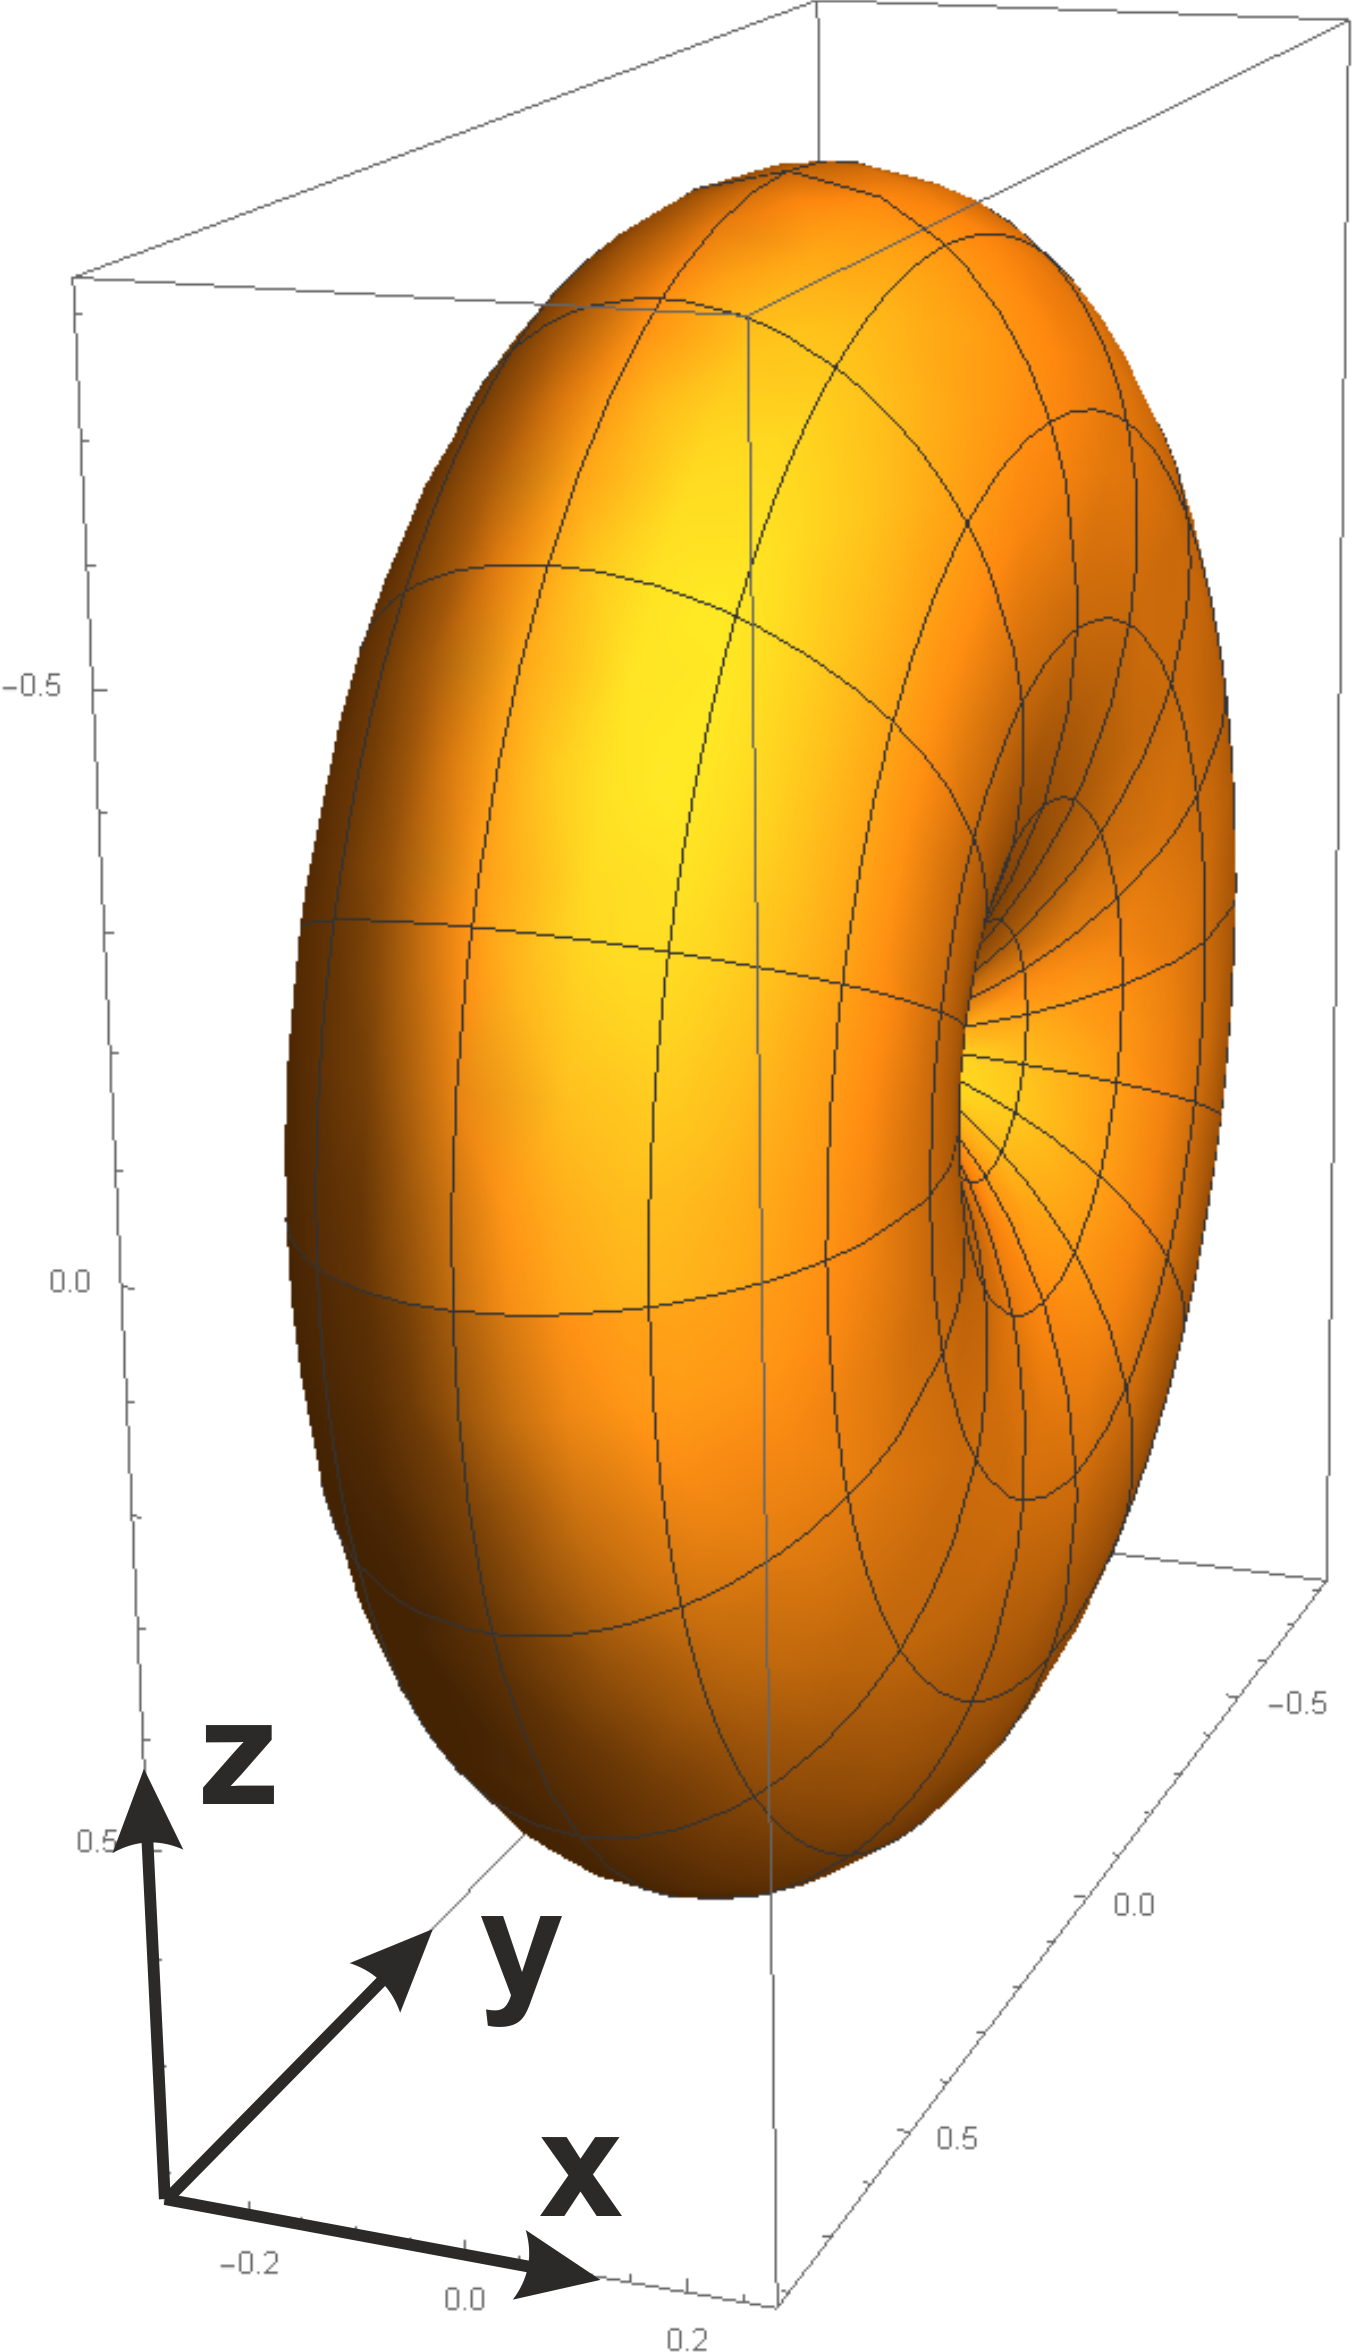
\includegraphics[width=0.4\textwidth]{../images/form_factor/cylindrical_obj/pOnsager(-3).png}}
\caption{Orientation distributions are are all independent on $\phi$ and have for $\kappa>0$ a positive order parameter, i.e. the most probable orientation is in the $\mathbf{x}$-direction and for $\kappa<0$ a negative order parameter, i.e. the most probable orientation lies in the $\mathbf{zy}$-plane}
\label{fig:pOnsager3D}
\end{figure}

\begin{table}[htp]
\centering
\caption{Values for $\kappa$ to obtain certain order parameters $S_2(\kappa)$ for the different orientation distributions $p(\theta,\phi,\kappa)$.}
\label{tab:kappas}
\begin{tabular}{|l|llllllllll|}
\toprule
\diagbox{$p(\theta,\phi,\kappa)$}{$S_2(\kappa)$}  & -0.45    & -0.4    & -0.2    & 0 & 0.2    & 0.4    & 0.6    & 0.8    & 0.9    & 0.95    \\ \midrule
Gauss       & -3.739 & -1.62  & -1.128 & 0 & 0.83  & 1.220 & 1.686 & 2.576 & 3.762 & 5.4    \\
Boltzmann   & -7.141 & -4.59  & -1.431 & 0 & 1.114 & 2.218 & 3.581 & 5.989 & 9     & 13.08 \\
Maier-Saupe & -15    & -7.49  & -1.874 & 0 & 1.367 & 2.709 & 4.444 & 8.241 & 15.59 & 30.54 \\
Onsager     & -28.43 & -13.35 & -2.918 & 0 & 2.042 & 3.629 & 6.313 & 13.92 & 28.96 & 58.99 \\
Heavyside   & -3.108 & -2.157 &	-1.129 & 0 & 0.794 & 0.982 & 1.267 & 1.868 & 2.692 & 3.840 \\
Hayter-Penfold   & $\varnothing$ & $\varnothing$&	$\varnothing$ & 0 & 3.008 & 6.269 & 10.93 & 20.8 & 34.91 & 55.64  \\ \bottomrule
\end{tabular}
\end{table}

\begin{figure}[htb]
\begin{center}
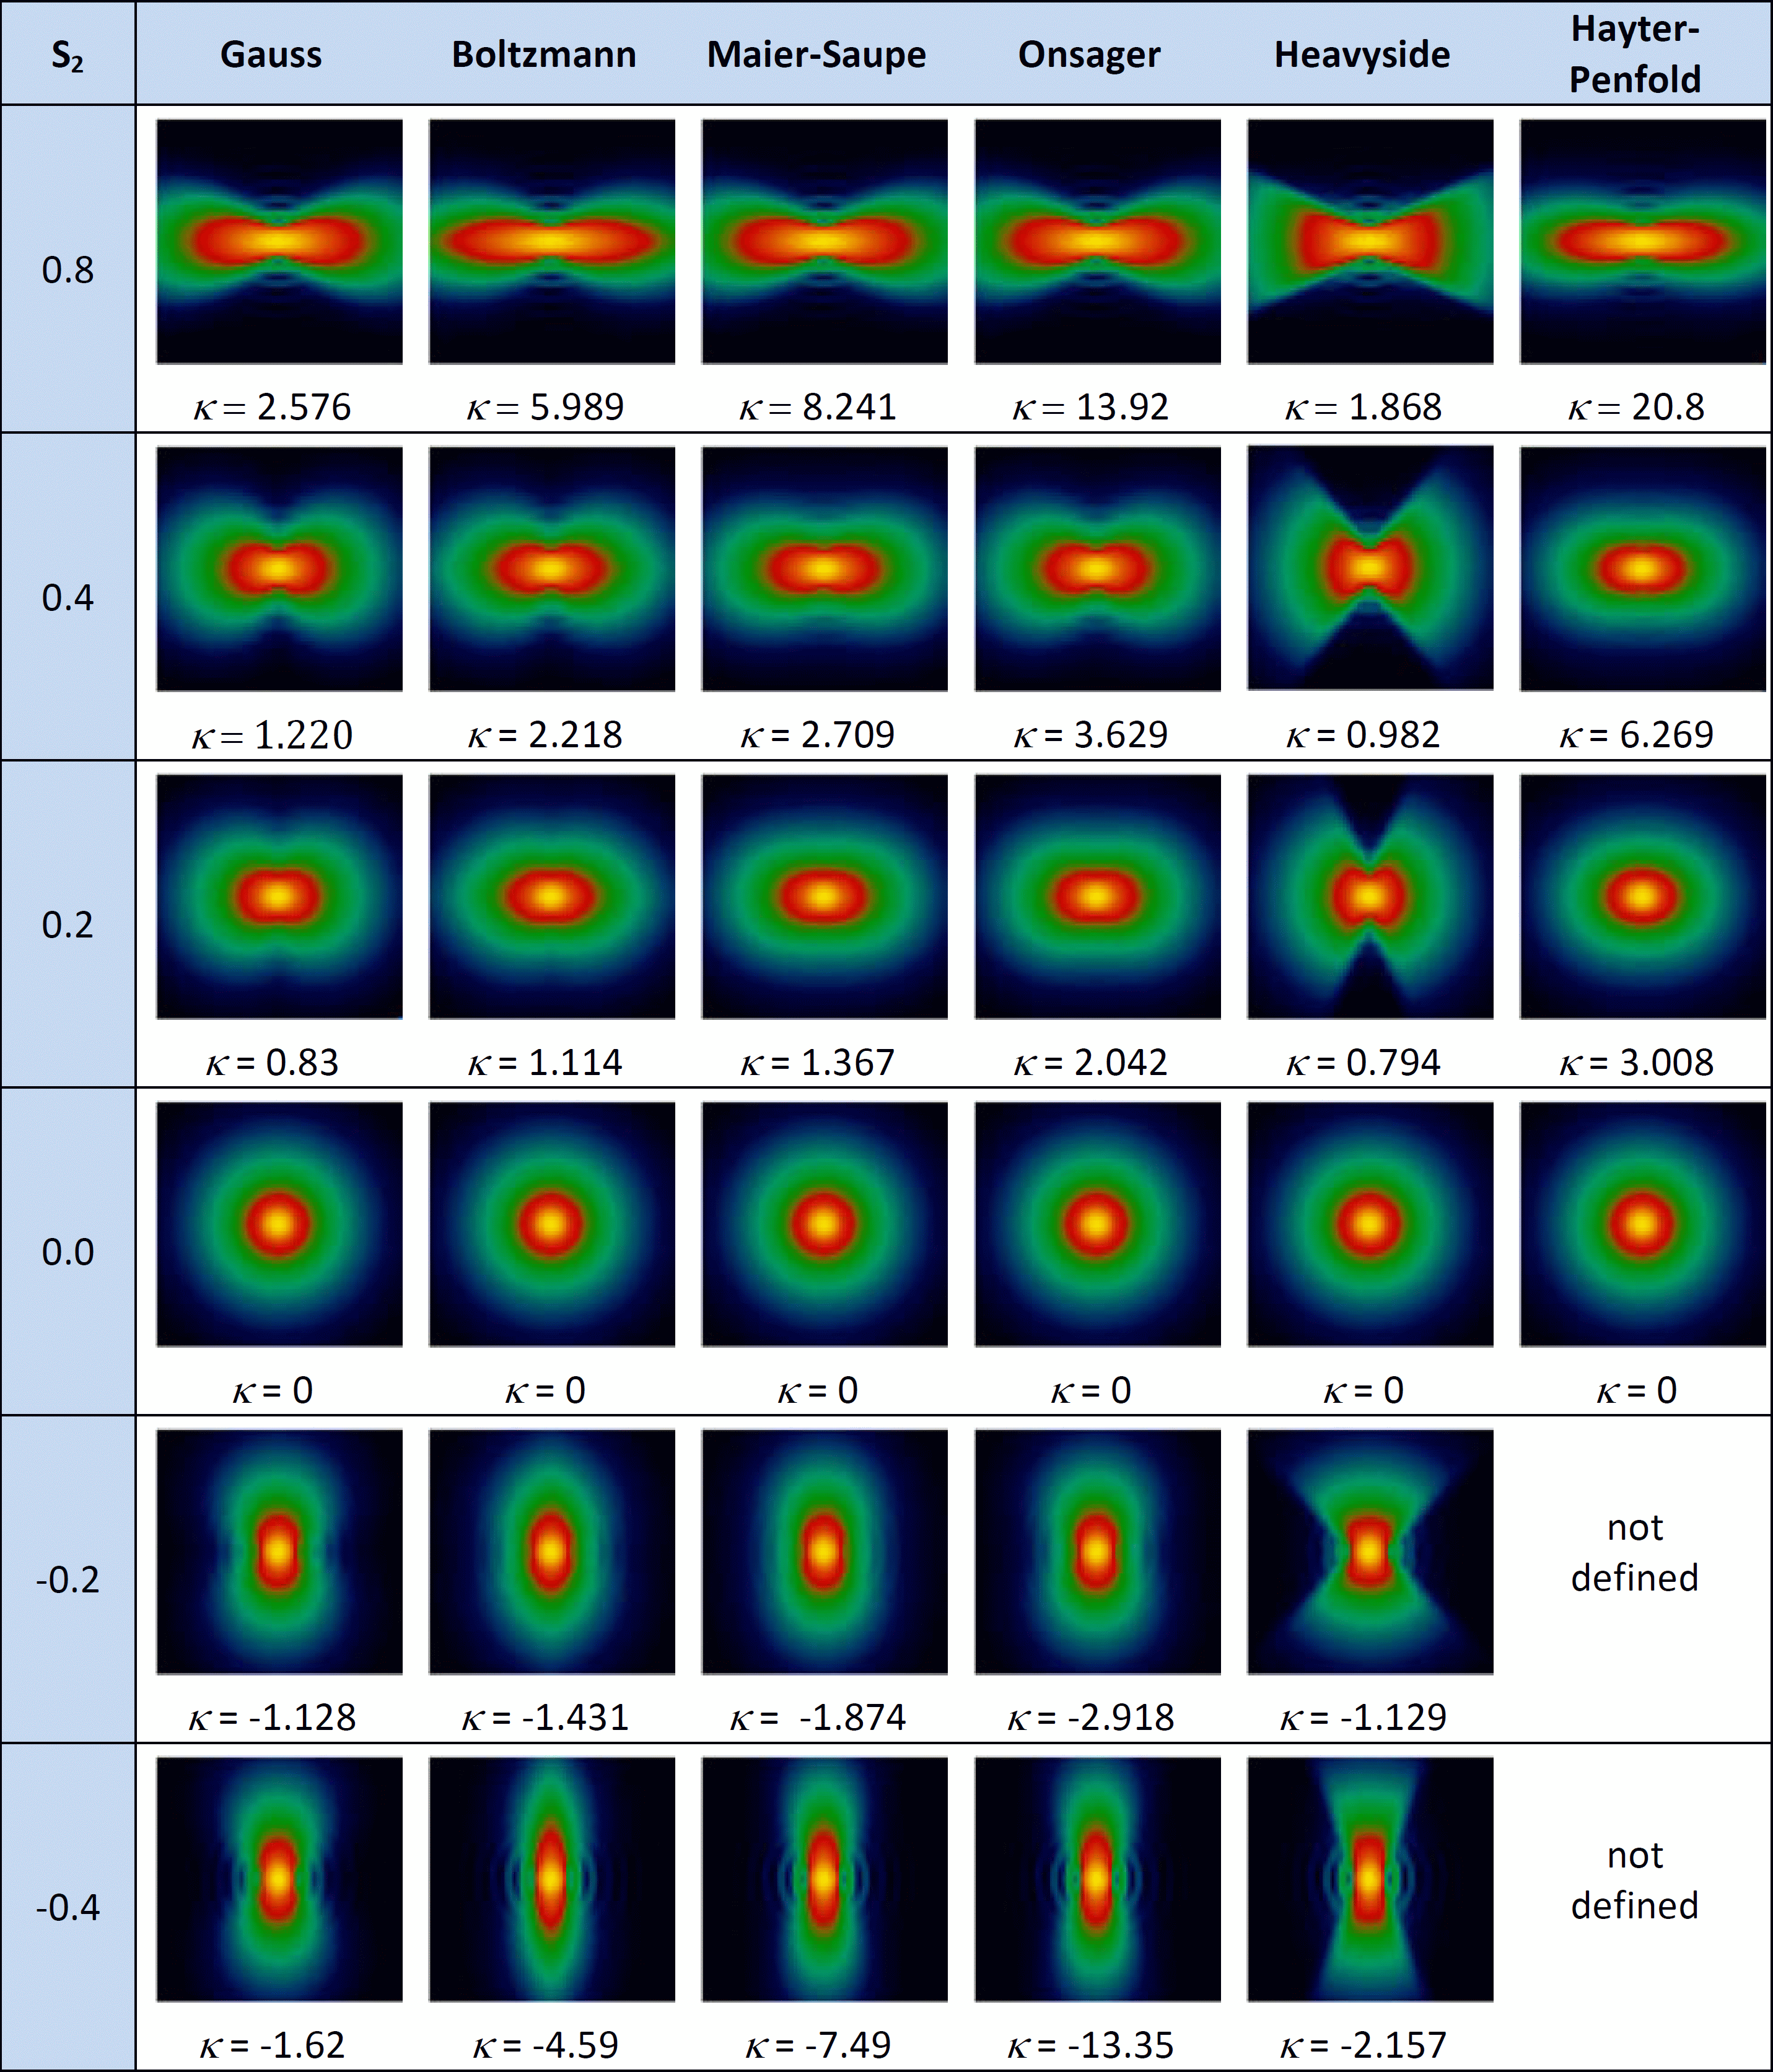
\includegraphics[width=0.95\textwidth]{../images/form_factor/cylindrical_obj/pXXXcomparison.png}
\end{center}
\caption{comparision of different orientation distributions with the same order parameter.}
\label{fig:S2_comparision}
\end{figure}

%Instead of assuming a
%special parametrization of $p(\theta)$ the orientation distribution was expanded in terms of
%Legendre polynomials $P_l(\cos(\theta))$
%\begin{align}
%p(\theta) & = \sum_{l=0,even}^\infty \frac{2l+1}{2} \left\langle P_l\right\rangle\, P_l(\cos(\theta))
%\end{align}
%Due to the symmetry $p(\theta)=p(\pi-\theta)$ all terms with odd values for $l$ are zero and only the
%even terms needs to be considered. For this form factor the first three terms up to $l=6$ are implemented.
%As $\int_0^\pi p(\theta) \sin\theta \, d\theta =1$ the zero order parameter is one $\left\langle P_0 %\right\rangle=1$.
%
%
%\vspace{5mm}
%
%\hspace{1pt}\\
%\underline{Input Parameters for model \texttt{partly aligned CylShell}:}\\
%\begin{description}
%\item[\texttt{R}] core radius $R$
%\item[\texttt{DR}] shell thickness $\Delta R$
%\item[\texttt{L}] cylinder length $L$
%\item[\texttt{eta\_core}] scattering length density $\eta_\text{core}$ of cylinder core
%\item[\texttt{eta\_shell}] scattering length density $\eta_\text{shell}$ of cylinder shell
%\item[\texttt{eta\_solv}] scattering length density $\eta_\text{solv}$ of solvent
%\item[\texttt{psi}] direction $\psi$ of the scattering vector in the plane of the detector
%\item[\texttt{P2}] order parameter $\langle P_2\rangle$
%\item[\texttt{P4}] order parameter $\langle P_4\rangle$
%\item[\texttt{P6}] order parameter $\langle P_6\rangle$
%\end{description}

%\begin{figure}[htb]
%\begin{center}
%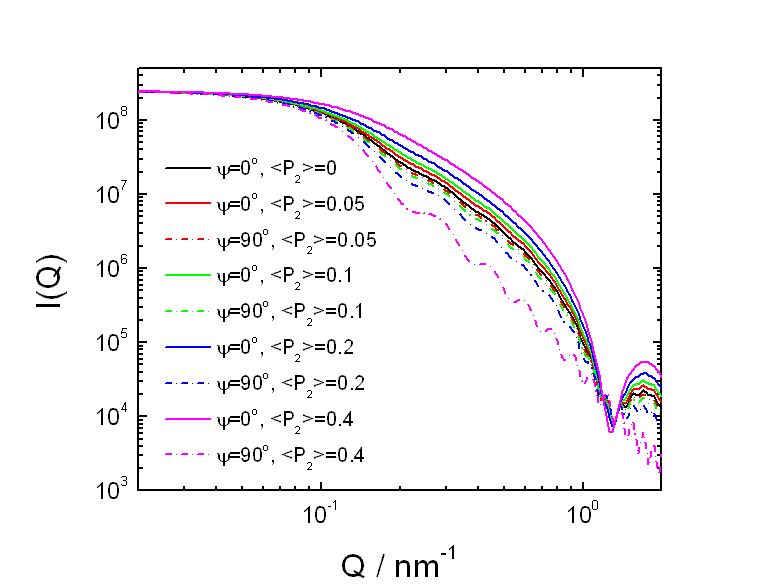
\includegraphics[width=0.786\textwidth,height=0.558\textwidth]{../images/form_factor/cylindrical_obj/partly_aligned_CylShell.png}
%\end{center}
%\caption{Scattering curve for partly aligned discs with radius $R=20$nm, $L=5$nm, $\Delta R=0$nm,
%and $\left\langle P_2 \right\rangle=$0, 0.05, 0.1, 0.2, and 0.4. Higher order parameters are set
%zero. $I(Q)$ is calculated for $\psi=0^\circ$ and $\psi=90^\circ$.}
%\label{fig:partly_aligned_CylShell}
%\end{figure}


%%%%%%%%%%%%%%%%%%%%%%%%%%%%%%%%%%%%%%%%%%%%%%%%%%%%%%%%%%%%%%%%%%%%%%%%%%%%%%%%%%%%%%%%%%%%
%\newpage
%\subsection{aligned cylindrical shell}
%\label{sect:alignedCylShell}
%\hspace{1pt}\\

\newpage
\subsubsection{Maier-Saupe orientation distribution} ~\\

\begin{align}
p(\theta,\phi;\kappa) & = \frac{1}{c_\mathrm{MS}}\exp\left(\kappa \cos^2\theta\right)
\end{align}
with
\begin{align}
c_\mathrm{MS} &=
\begin{cases}
\displaystyle
4\pi\exp(\kappa) \frac{\mathrm{D}\left(\sqrt{\kappa}\right)}{\sqrt{\kappa}}   &\mathrm{for~} \kappa > 0 \\[5mm]
\displaystyle
2\pi \sqrt{\pi} \frac{\mathrm{erf}\left(\sqrt{\abs{\kappa}}\right)}{\sqrt{\abs{\kappa}}}  &\mathrm{for~} \kappa < 0 \\[2mm]
\displaystyle
4\pi                                                                                      &\mathrm{for~} \kappa = 0
\end{cases}
\end{align}
with $D(x)$ being Dawson's integral $D(x)=e^{-x^2}\int_0^x e^{y^2} \mathrm{d}y = \frac12\sqrt{\pi}e^{-x^2}\mathrm{erfi}(x)$
%%%%%%%%%%%%%%%%%%%%%%%%%%%%%%%%%%%%%%%%%%%%%%%%%%%%%%%%%%%%%%%%%%%%%%%%%%%%%%%%%%

\newpage
\subsubsection{Onsager orientation distribution} ~\\

\begin{align}
p(\theta,\phi;\kappa) & =
\begin{cases} \displaystyle
\frac{\kappa \cosh\left(\kappa \cos(\theta)\right)}{4\pi \sinh(\kappa)}      &\mathrm{for~} \kappa \geq 0 \\[5mm]
 \displaystyle
\frac{\cosh\left(\abs{\kappa} \sin(\theta)\right)}{2\pi^2 L_1(\abs{\kappa})}  &\mathrm{for~} \kappa < 0
\end{cases}
\end{align}
where $L_\nu(x)$ is the modified Struve function.

%%%%%%%%%%%%%%%%%%%%%%%%%%%%%%%%%%%%%%%%%%%%%%%%%%%%%%%%%%%%%%%%%%%%%%%%%%%%%%%%%%

\newpage
\subsubsection{Boltzmann orientation distribution} ~\\

\begin{align}
p(\theta,\phi;\kappa) & =
\begin{cases}
\displaystyle
\frac{1}{2\pi c_\mathrm{B}}\exp\left(-\theta\kappa\right) & \mathrm{for~}  \theta \leq \frac{\pi}{2}\\[5mm]
\displaystyle
\frac{1}{2\pi c_\mathrm{B}}\exp\left(-(\pi-\theta)\kappa\right) & \mathrm{for~}  \theta > \frac{\pi}{2}
\end{cases}
\end{align}
with
\begin{align}
c_\mathrm{B} &= \frac{2\left(1-\kappa \exp\left(-\frac{\pi}{2}\kappa\right)\right)}{\kappa^2+1}
\end{align}
%%%%%%%%%%%%%%%%%%%%%%%%%%%%%%%%%%%%%%%%%%%%%%%%%%%%%%%%%%%%%%%%%%%%%%%%%%%%%%%%%%

\newpage
\subsubsection{Gaussian orientation distribution}
\label{sect:ShearedCylinderGaussian}
~\\
\begin{align}
p(\theta,\phi;\kappa) & =
\begin{cases}
\displaystyle
\frac{1}{2\pi c_\mathrm{G}}\exp\left(-\theta^2\kappa^2\right) & \mathrm{for~} \kappa \geq 0 \mathrm{~and~} \theta \leq \frac{\pi}{2}\\[5mm]
\displaystyle
\frac{1}{2\pi c_\mathrm{G}}\exp\left(-\left(\pi-\theta\right)^2\kappa^2\right) & \mathrm{for~} \kappa \geq 0 \mathrm{~and~} \theta > \frac{\pi}{2}\\[5mm]
\displaystyle
\frac{1}{2\pi c_\mathrm{G}}\exp\left(-\left(\frac{\pi}{2}-\theta\right)^2\abs{\kappa}^2\right) & \mathrm{for~} \kappa < 0
\end{cases}
\end{align}
with
\begin{align}
c_\mathrm{G} & =
\begin{cases}\displaystyle
\frac{D\left(\kappa/2\right)}{\kappa}
           +\frac{\sqrt{\pi}}{2\kappa} e^{-\frac{1}{4\kappa^2}} \Re\left(\mathrm{cerfi}\left(-\frac{1}{2\kappa}+\imath\frac{\pi}{2}\kappa\right) \right)& \mathrm{for~} \kappa \geq 0 \\[5mm]
\displaystyle
\frac{\sqrt{\pi}}{\abs{\kappa}} e^{-\frac{1}{4\kappa^2}} \Im\left(\mathrm{cerfi}\left(-\frac{1}{2\abs{\kappa}}+\imath\frac{\pi}{2}\abs{\kappa}\right) \right) & \mathrm{for~} \kappa < 0
\end{cases}
\end{align}
%%%%%%%%%%%%%%%%%%%%%%%%%%%%%%%%%%%%%%%%%%%%%%%%%%%%%%%%%%%%%%%%%%%%%%%%%%%%%%%%%%

\newpage
\subsubsection{ShearedCylinderHeaviside} ~\\

\begin{align}
p(\theta,\phi;\bar{\theta}) & = \Theta[\theta-\bar{\theta}] \\
\cos\gamma^\pm & = \sin\theta\cos\phi\cos\psi\pm\cos\theta\sin\psi
\end{align}

%\item[ShearedCylinderMaierSaupe] ~\\
%\begin{align}
%p(\theta,\phi;\bar{\theta}) & = \exp[\cos^2(\theta/\bar{\theta})]-1 \\
%\cos\gamma^\pm              & = \sin\theta \cos\phi \sin\psi \pm \cos\theta\cos\phi
%\end{align}
%
%\item[ShearedCylinderOnsager] ~\\
%\begin{align}
%p(\theta,\phi;\bar{\theta}) & = \exp[-\sin(\theta/\bar{\theta})] \\
%\cos\gamma^\pm              & = \sin\theta \cos\phi \sin\psi \pm \cos\theta\cos\phi
%\end{align}

